This chapter describes the Winoground \cite{thrush2022winoground} dataset (\cref{sec:winoground_dataset}) and explains the metrics used for evaluation. We also describe a series of previous and new experiments performed over the Winoground dataset using state-of-the-art vision and language models (\cref{sec:winoground_experiments_results}). The Winoground dataset does not contain a training split, and therefore the experiments are conducted in a zero-shot fashion, where the models are trained on different datasets, and tested on Winoground.

The original Winoground paper included zero-shot experiments with many pre-trained SOTA systems, and they concluded that, surprisingly, none of them does much better than chance \cite{thrush2022winoground}. From these experiments, the authors conclude that SOTA models are not as skilled at visio-linguistic compositional reasoning as we might have hoped.

In this work, we extended the previous experiments with new models that obtained better results than those reported in the original paper. In previous experiments, only pre-trained models are tested. We extend this by testing some models that are fine-tuned for specific tasks such as image-text retrieval and visual reasoning. We compare pre-trained versions with fine-tuned versions of the same models and find out that fine-tuning helps.

\section{Winoground Dataset} \label{sec:winoground_dataset}

The Winoground dataset \cite{thrush2022winoground} comprises 400 examples that probe different aspects of visio-linguistic compositional reasoning. Each example contains two images and two captions, the goal
is to match them correctly. Both captions contain a completely identical set of words or morphemes in a different order. Figures \cref{fig:winoground-examples,fig:winoground-examples-linguistic,fig:winoground-examples-visual} show some examples. The dataset was created by expert annotators by designing captions and finding images on Getty Images. All examples are labeled with \textbf{linguistic tags} and some include \textbf{visual tags}. See \cref{tab:stats-tag-subset} for linguistic and visual tag counts.

\begin{table}[ht]
\centering
\begin{tabular}{lrr}
\toprule
 Category & Tag    &   Count \\
\midrule
 %All Examples & 400\\
 & Object   &     141 \\
 Linguistic$_\text{swap-dep.}$ & Relation &     233 \\
 & Both &      26 \\\midrule
 Linguistic$_\text{swap-indep.}$ & 1 Main Pred & 292 \\
 & 2 Main Preds & 108 \\\midrule
 & Symbolic &  41 \\
 Visual & Series &  31 \\
 & Pragmatics &  24\\
\bottomrule
\end{tabular}
\caption{Linguistic and visual tag counts in the Winoground dataset. Every example has a linguistic tag; only examples that contain visual phenomena have visual tags.}
\label{tab:stats-tag-subset}
\end{table}

On the one hand, there are 70 \textbf{linguistic tags} in total, which can be split into three groups: Object, Relation and Both. \textbf{Object} swaps consist in swapping noun phrases that refer to objects. \textbf{Relation} swaps reorder words that refer to objects such as verbs, adjectives, prepositions and adverbs. \textbf{Both} swaps involve changing both relations and objects. The annotators also tagged examples for \textbf{how many main predicates} were in the captions, which is independent of the swap type. See \cref{fig:winoground-examples,fig:winoground-examples-linguistic} for examples of linguistic tags.

\begin{figure}[ht]
\centering
    \begin{minipage}[t]{.30\textwidth}
        \begin{subfigure}[t]{\textwidth}
        \centering
        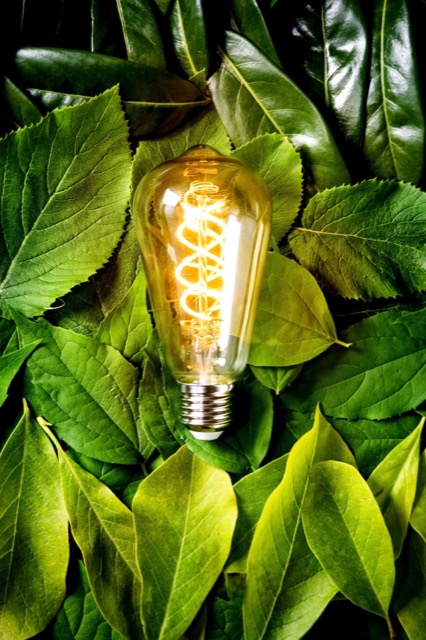
\includegraphics[height=3cm]{ex_155_img_0.png}
        \caption{[some plants] surrounding [a lightbulb]}
        \end{subfigure}\\
        \begin{subfigure}[t]{\textwidth}
        \centering
        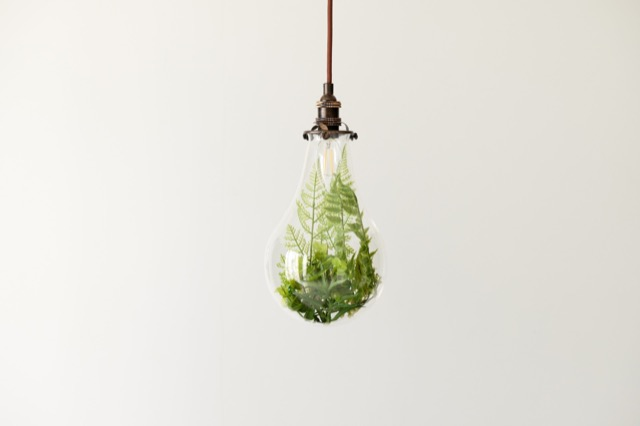
\includegraphics[height=3cm]{ex_155_img_1.png}
        \caption{[a lightbulb] surrounding [some plants]}
        \end{subfigure}%
        \caption*{\textit{Object}}
    \end{minipage}
    \hfill
    \begin{minipage}[t]{.30\textwidth}
        \begin{subfigure}[t]{\textwidth}
        \centering
        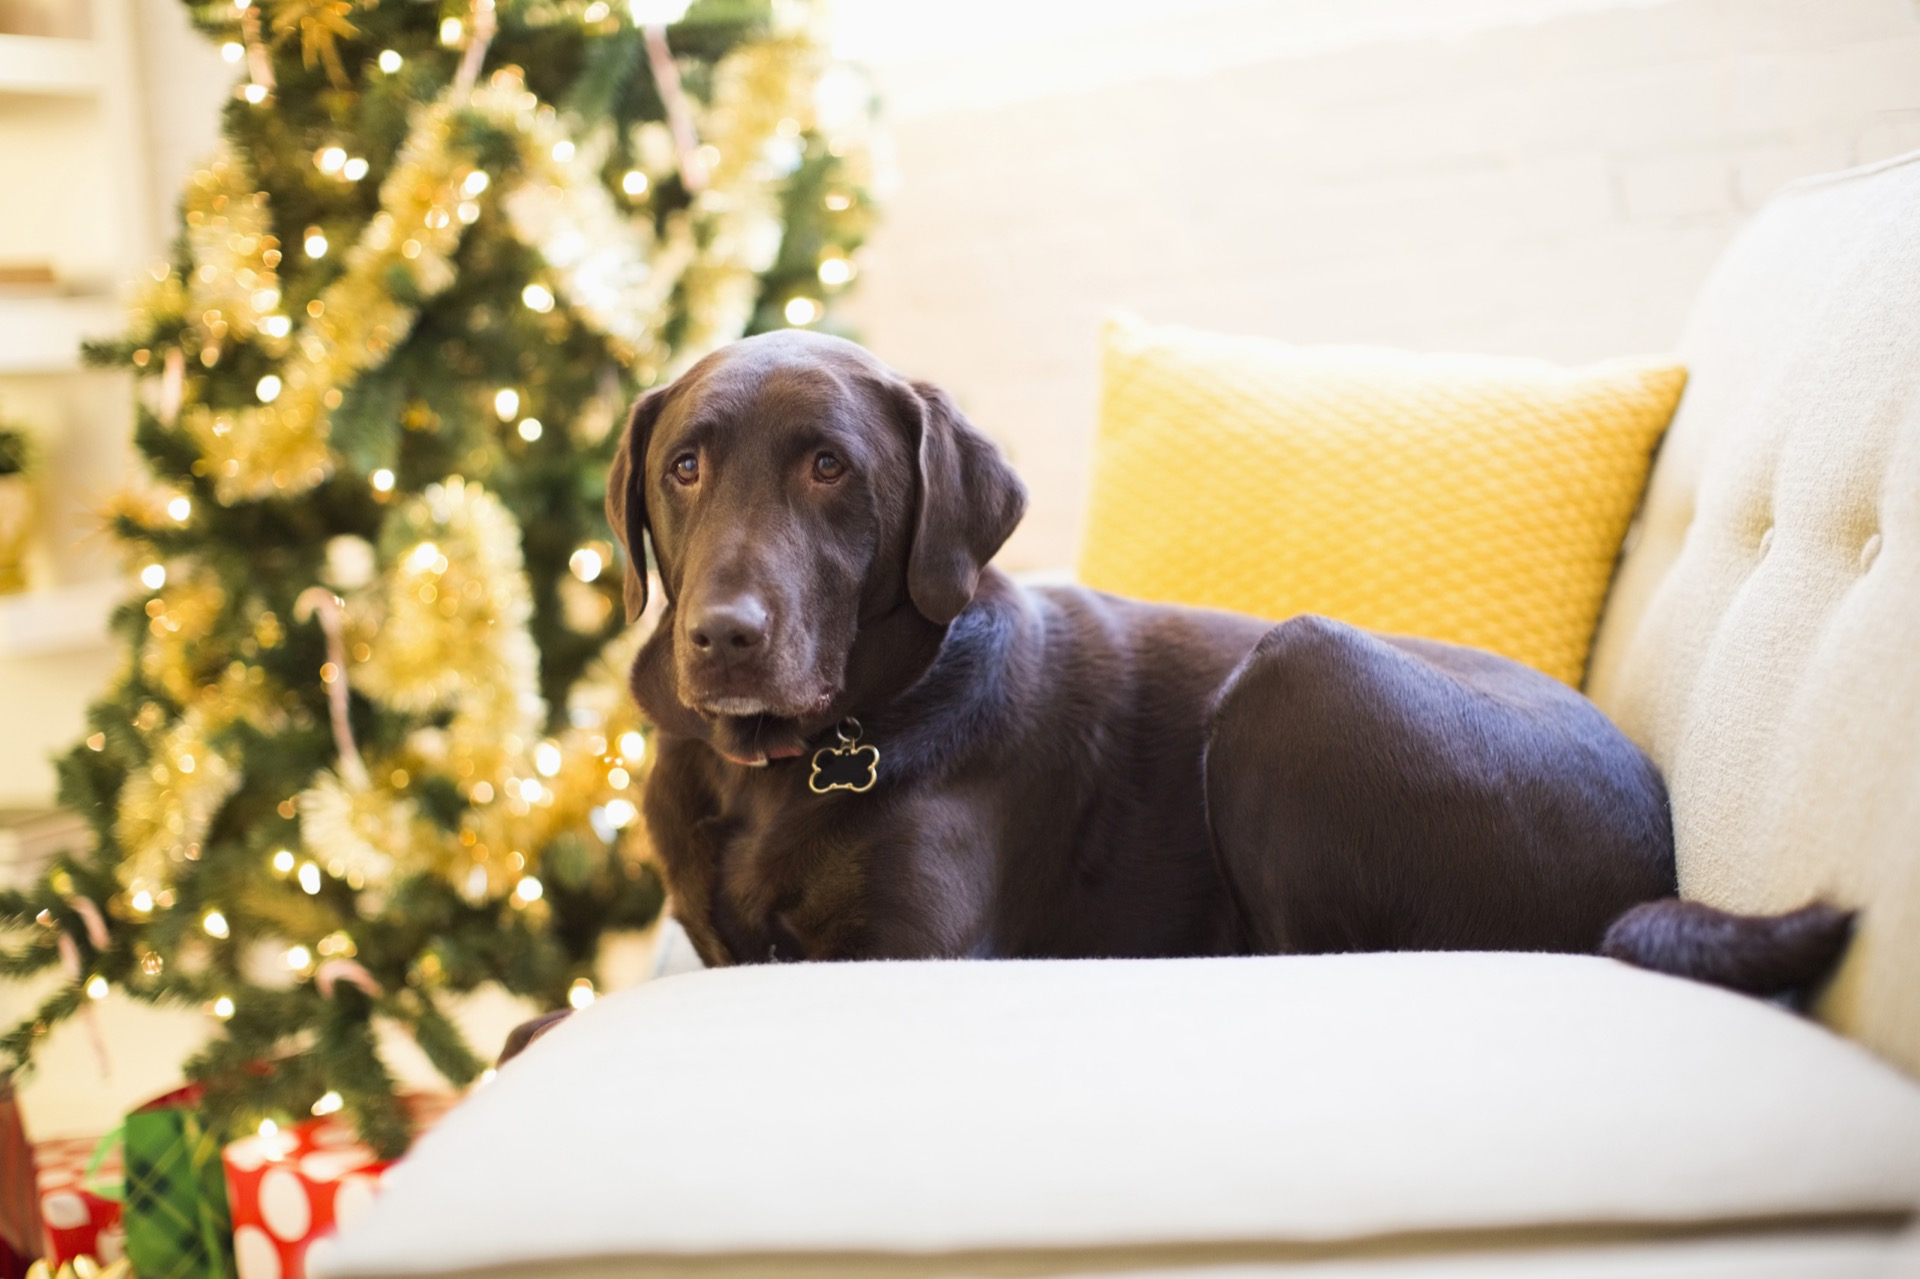
\includegraphics[height=3cm]{ex_29_img_0.png}
        \caption{a [brown] dog is on a [white] couch}
        \end{subfigure}\\
        \vspace{10pt}
        \begin{subfigure}[t]{\textwidth}
        \centering
        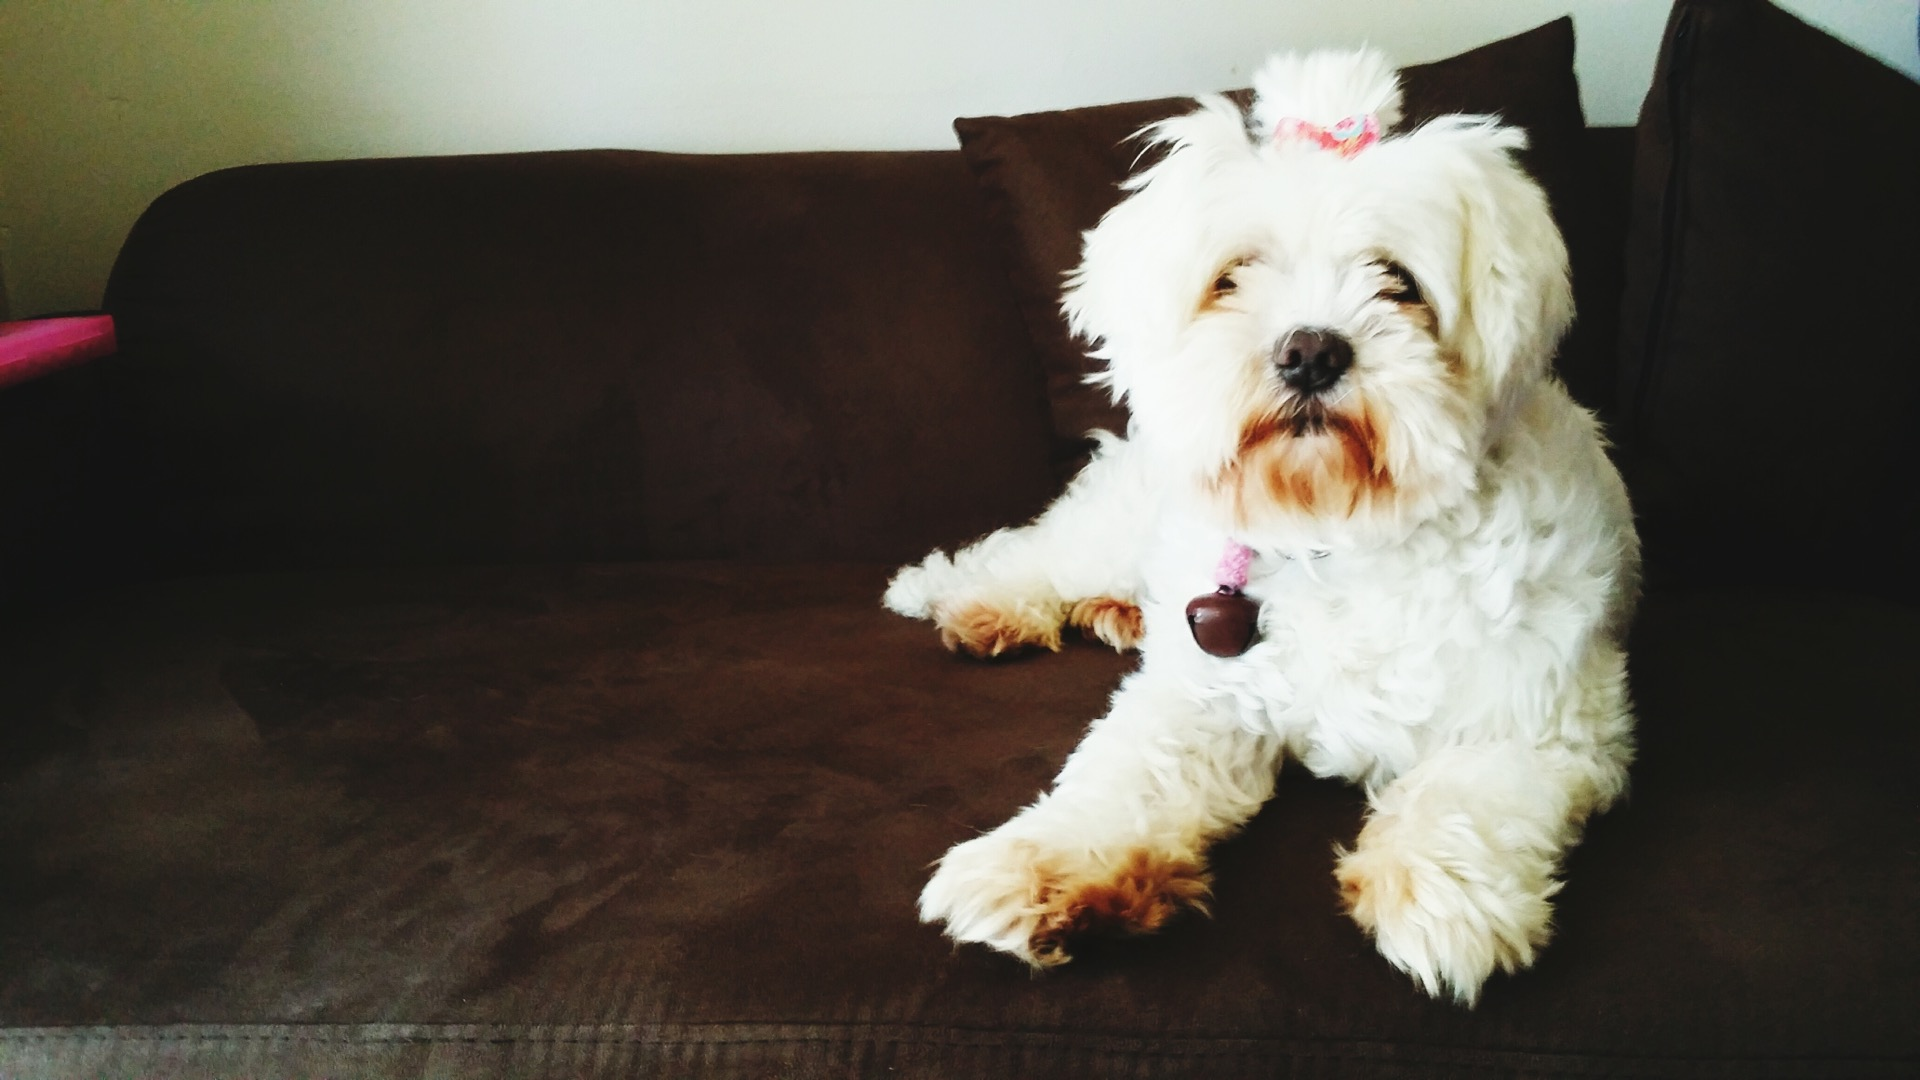
\includegraphics[height=3cm]{ex_29_img_1.png}
        \caption{a [white] dog is on a [brown] couch}
        \end{subfigure}% 
        \vspace{10pt}
        \caption*{\textit{Relation}}
    \end{minipage}
    \hfill
    \begin{minipage}[t]{.30\textwidth}
        \begin{subfigure}[t]{\textwidth}
        \centering
        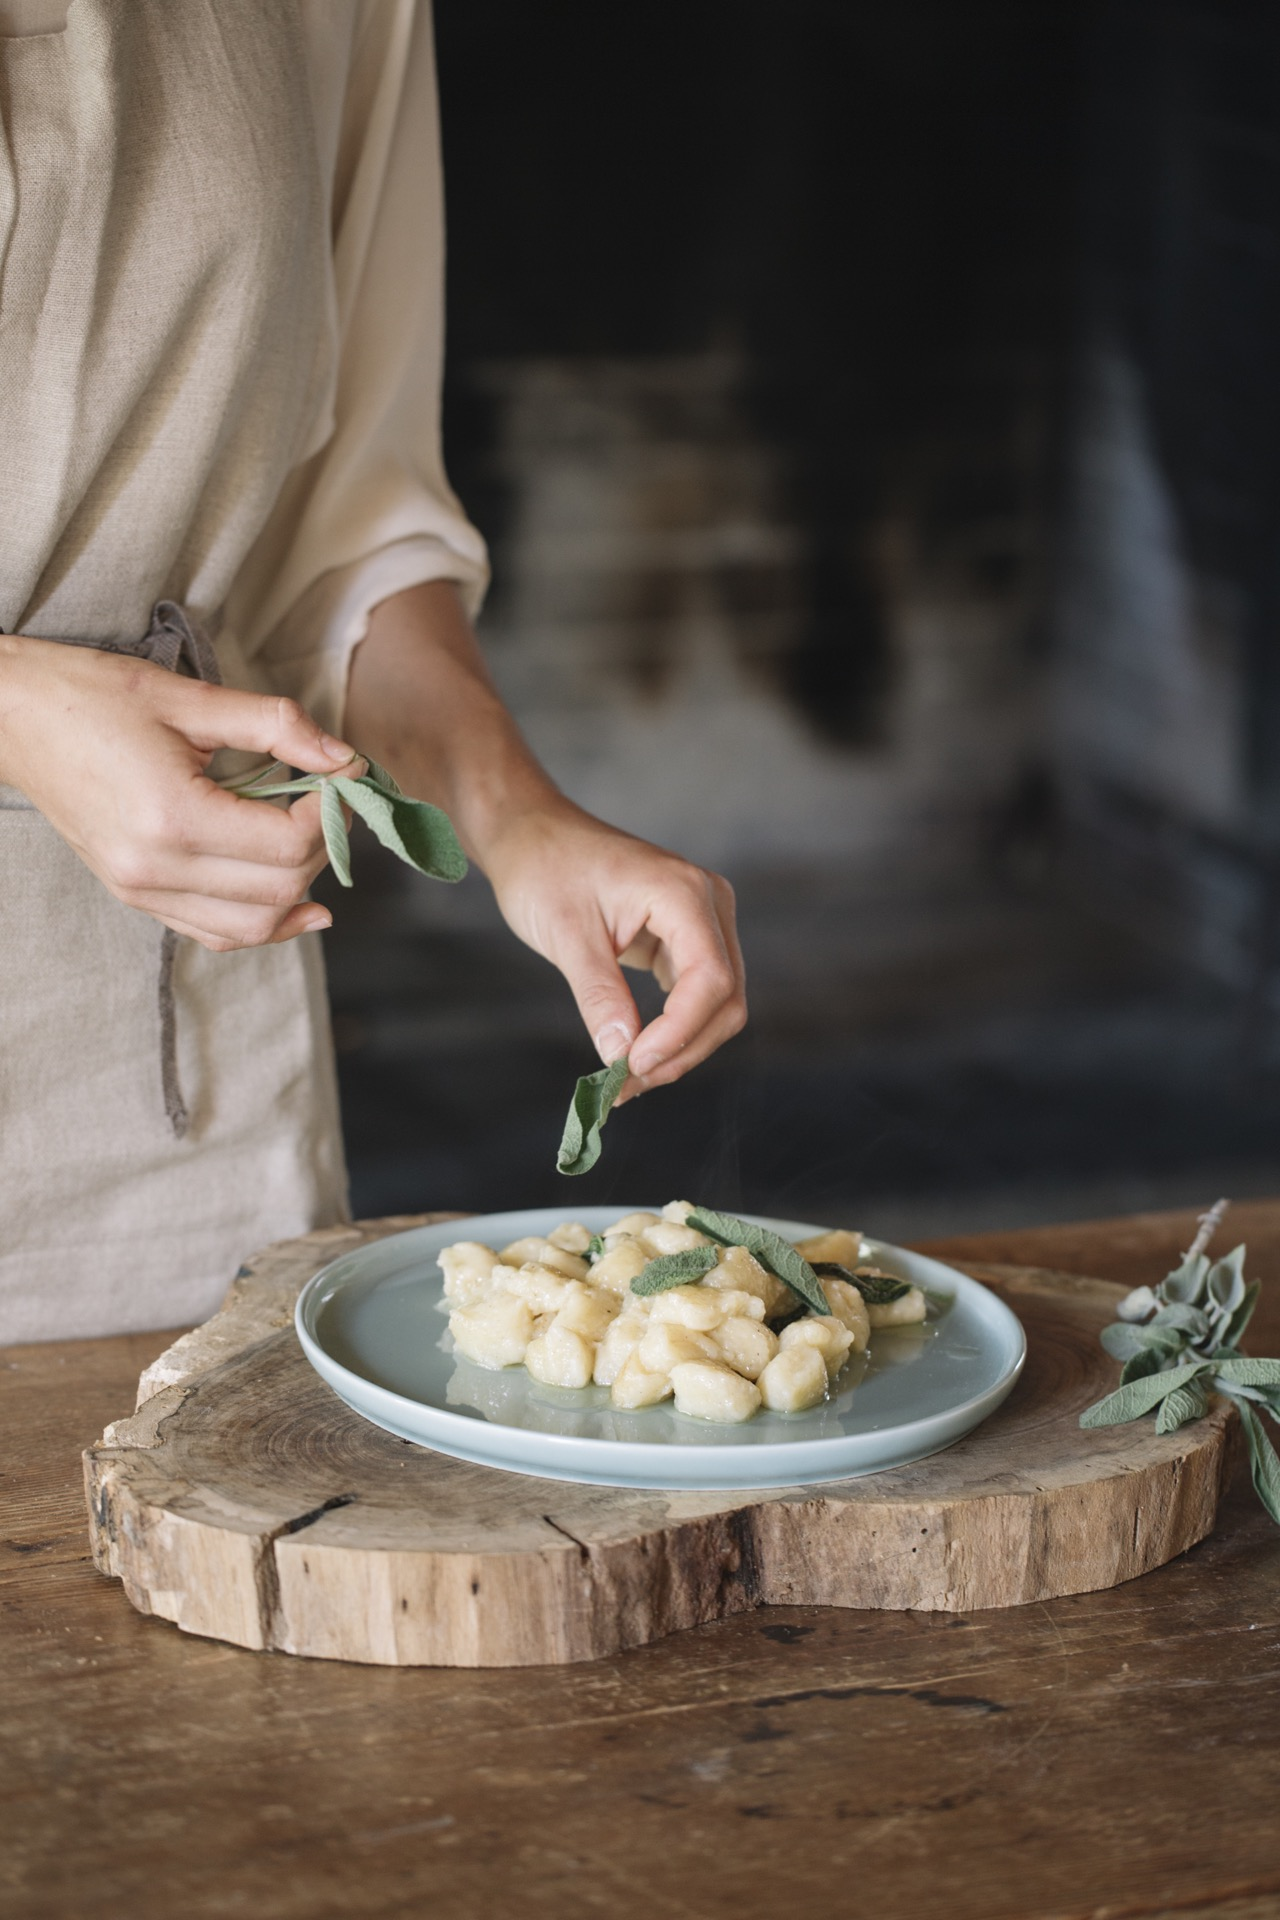
\includegraphics[height=3cm]{ex_118_img_0.png}
        \caption{[circular] food on [heart-shaped] wood}
        \end{subfigure}\\
        \begin{subfigure}[t]{\textwidth}
        \centering
        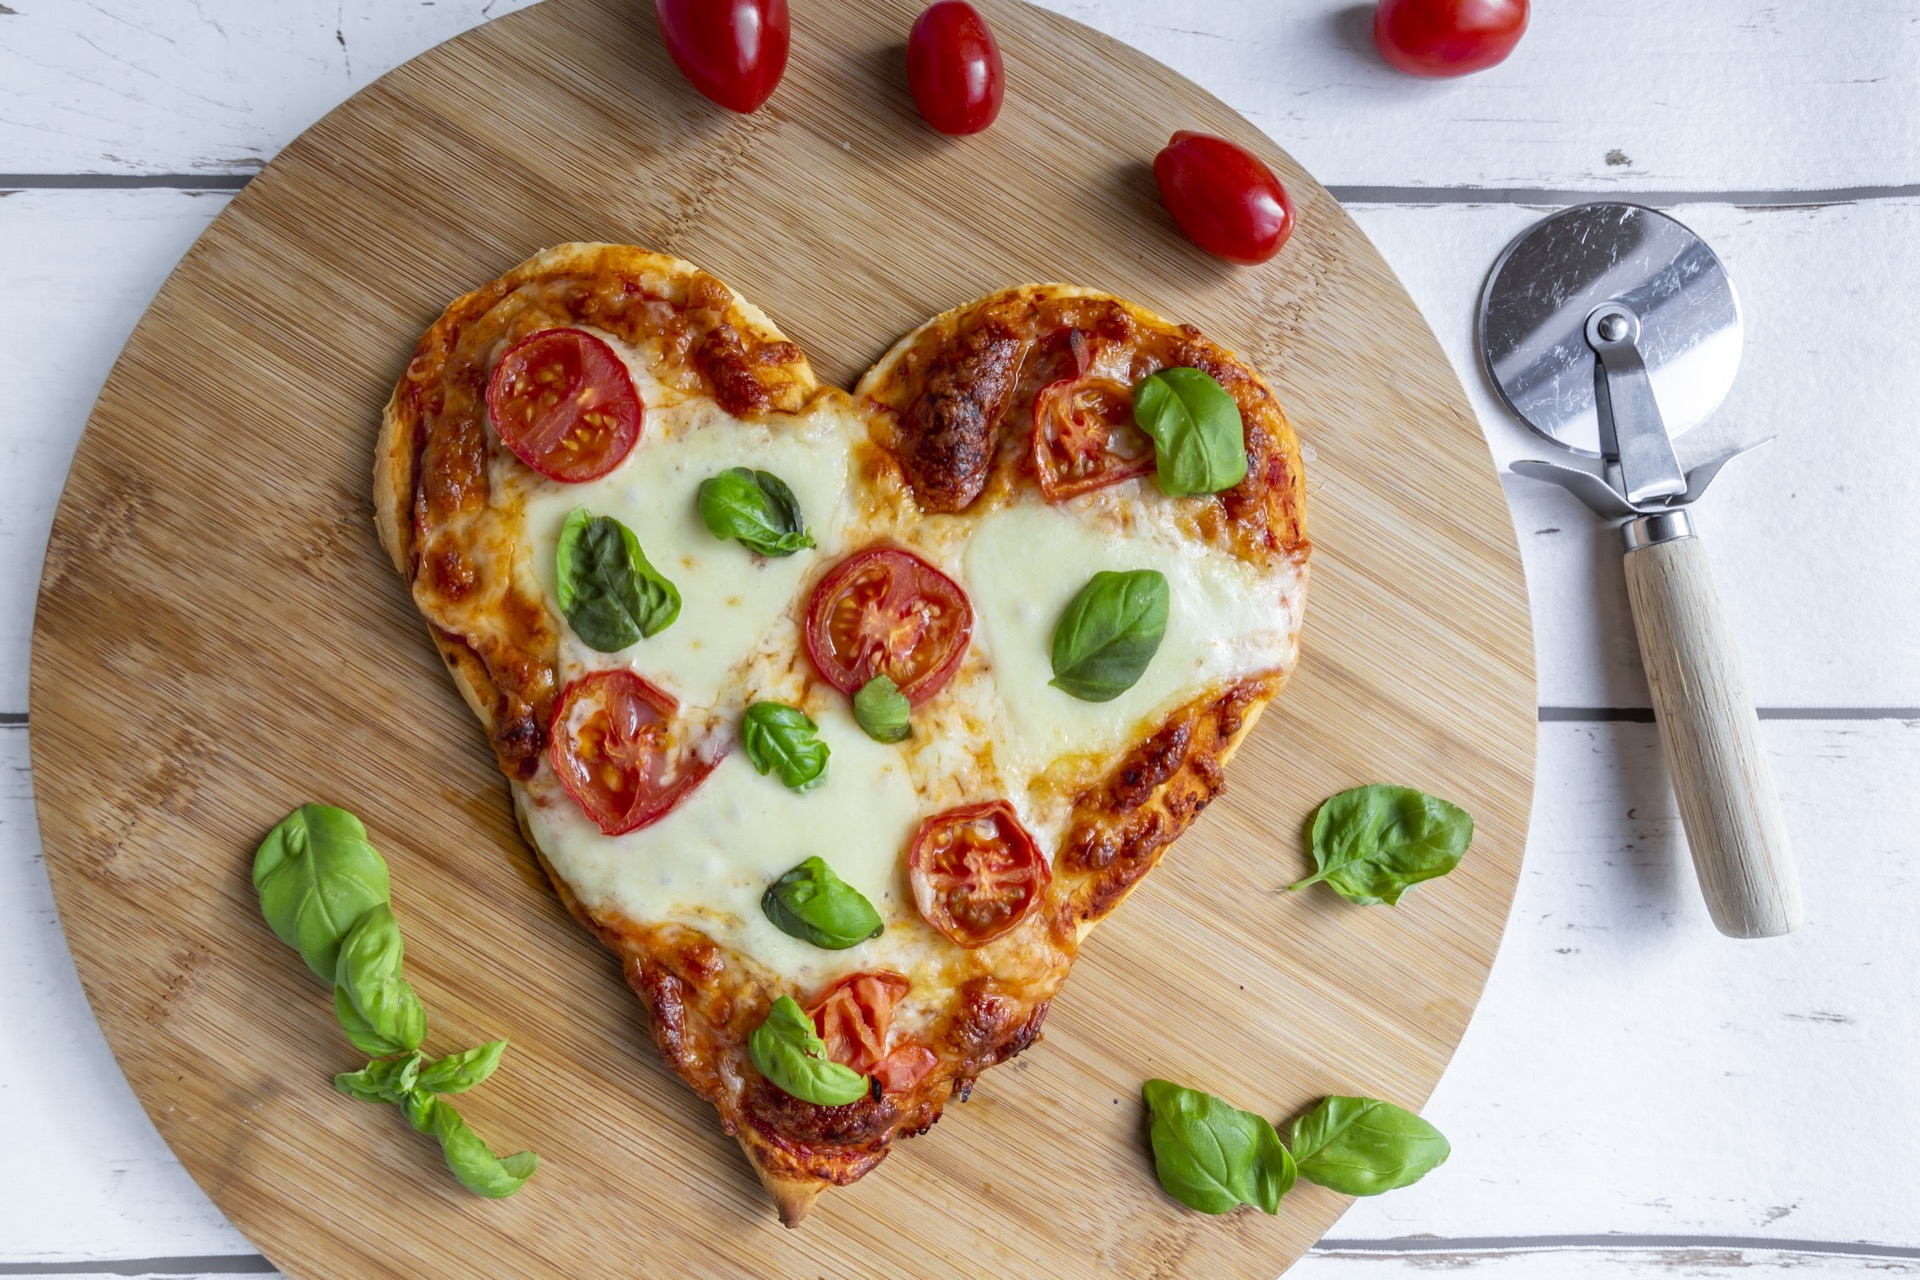
\includegraphics[height=3cm]{ex_118_img_1.png}
        \caption{[heart-shaped] food on [circular] wood}
        \end{subfigure}%
        \caption*{\textit{Relation}}
    \end{minipage}%
    \caption{Examples from the Winoground dataset for the swap-dependent linguistic tags \textit{Object}, \textit{Relation} and \textit{Relation} from left to right. They are additionally tagged with 1 main predicate.}
    \label{fig:winoground-examples}
\end{figure}

\begin{figure}[ht]
\centering
    \begin{minipage}[t]{.30\textwidth}
        \begin{subfigure}[t]{\textwidth}
        \centering
        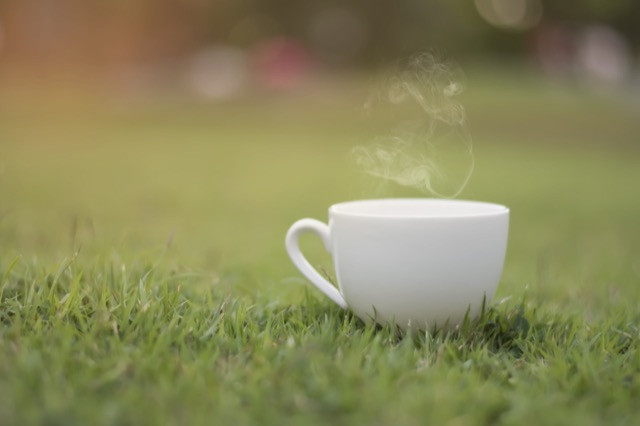
\includegraphics[height=3cm]{ex_14_img_0.png}
        \caption{there is [a mug] in [some grass]}
        \end{subfigure}\\
        \begin{subfigure}[t]{\textwidth}
        \centering
        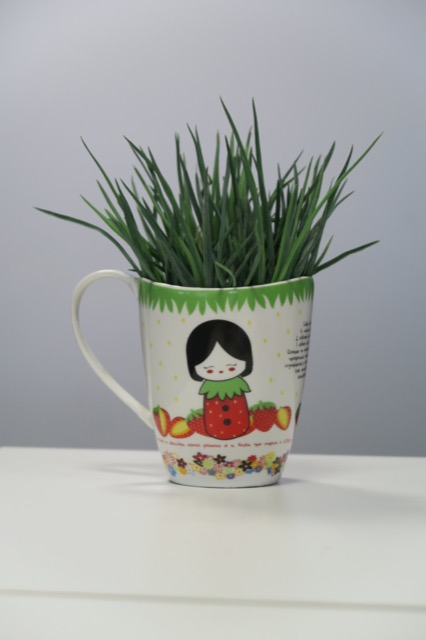
\includegraphics[height=3cm]{ex_14_img_1.png}
        \caption{there is [some grass] in [a mug]}
        \end{subfigure}%    
        \caption*{\textit{Object}}
    \end{minipage}
    \hfill
    \begin{minipage}[t]{.30\textwidth}
        \begin{subfigure}[t]{\textwidth}
        \centering
        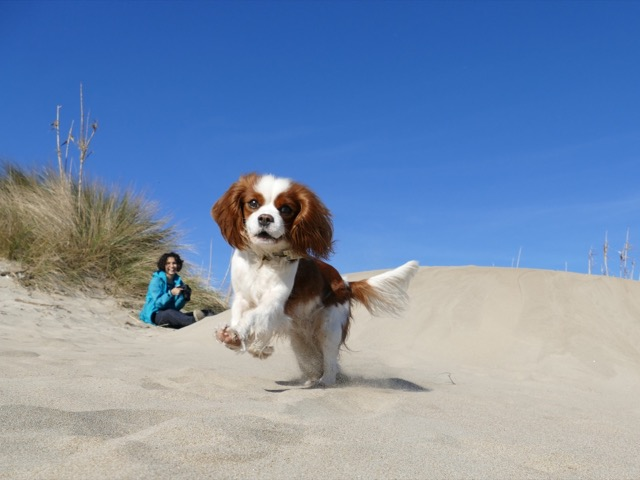
\includegraphics[height=3cm]{ex_21_img_0.png}
        \caption{a person [sits] and a dog [stands]}
        \end{subfigure}\\
        \begin{subfigure}[t]{\textwidth}
        \centering
        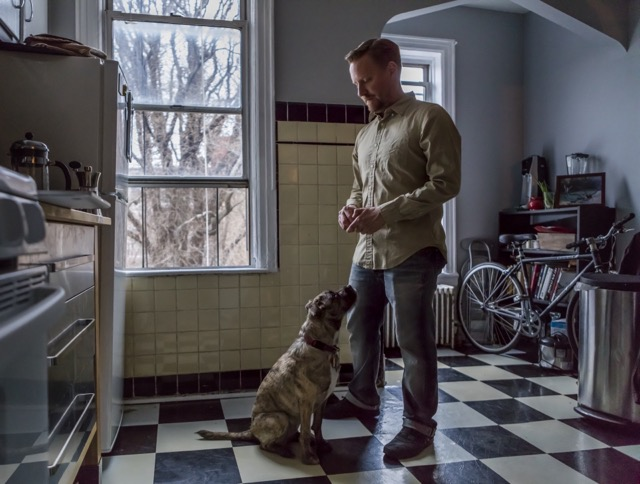
\includegraphics[height=3cm]{ex_21_img_1.png}
        \caption{a person [stands] and a dog [sits]}
        \end{subfigure}%    
        \caption*{\textit{Relation}}
    \end{minipage}
    \hfill
    \begin{minipage}[t]{.30\textwidth}
        \begin{subfigure}[t]{\textwidth}
        \centering
        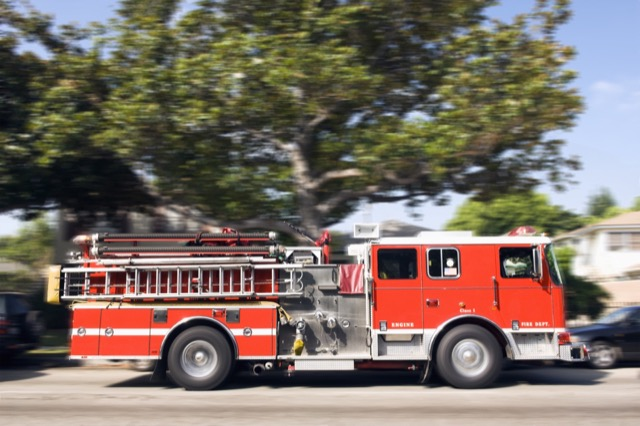
\includegraphics[height=3cm]{ex_72_img_0.png}
        \caption{it's a [fire] [truck]}
        \end{subfigure}\\
        \begin{subfigure}[t]{\textwidth}
        \centering
        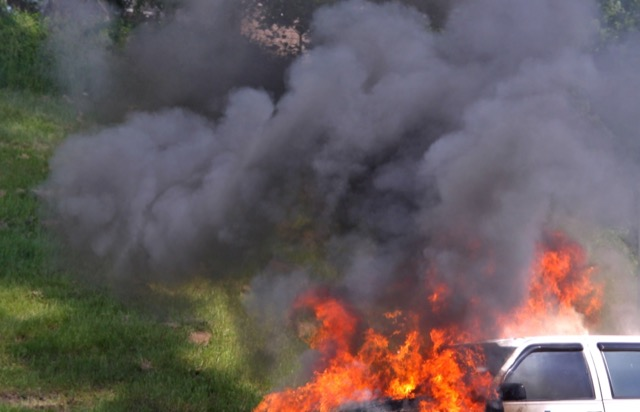
\includegraphics[height=3cm]{ex_72_img_1.png}
        \caption{it's a [truck] [fire]}
        \end{subfigure}%
        \caption*{\textit{Both}}
    \end{minipage}%
    \caption{Examples from the Winoground dataset for the swap-dependent linguistic tags \textit{Object}, \textit{Relation} and \textit{Both} from left to right. They are additionally tagged with 1, 2 and 1 main predicates from left to right.}
    \label{fig:winoground-examples-linguistic}
\end{figure}

On the other hand, there are three non-mutually exclusive \textbf{visual reasoning tags}: Pragmatics, Series and Symbolic. \textbf{Pragmatics} tag includes images that need to be interpreted non-literally. \textbf{Series} tag contains examples where both images come from the same photo series. \textbf{Symbolic} tag represents that the images include a symbolic representation. \cref{fig:winoground-examples-visual} shows examples of visual tags.

\begin{figure}[ht]
\centering
    \begin{minipage}{.30\textwidth}
        \begin{subfigure}{\textwidth}
        \centering
        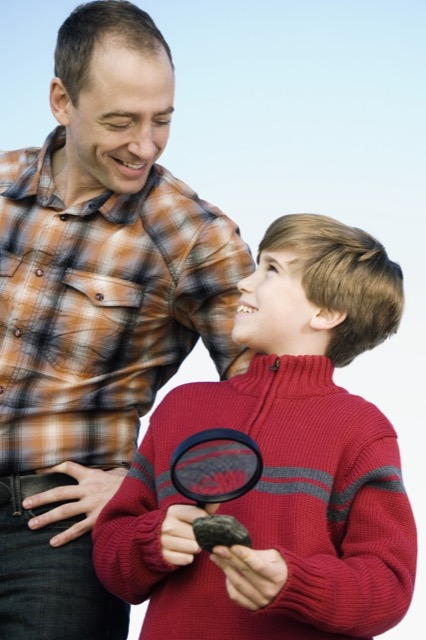
\includegraphics[height=3cm]{ex_75_img_0.png}
        \caption{the kid [with the magnifying glass] looks at them []}
        \end{subfigure}\\
        \begin{subfigure}{\textwidth}
        \centering
        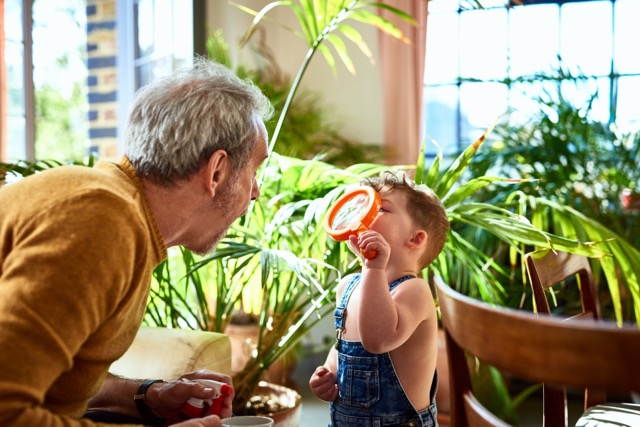
\includegraphics[height=3cm]{ex_75_img_1.png}
        \caption{the kid [] looks at them [with the magnifying glass]}
        \end{subfigure}%    
        \caption*{\textit{Pragmatics}}
    \end{minipage}
    \hfill
    \begin{minipage}{.30\textwidth}
        \begin{subfigure}{\textwidth}
        \centering
        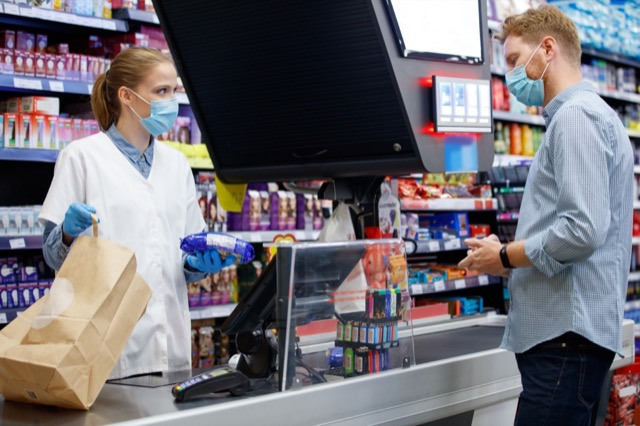
\includegraphics[height=3cm]{ex_27_img_0.png}
        \caption{the person with the ponytail [packs] stuff and other [buys] it}
        \end{subfigure}\\
        \begin{subfigure}{\textwidth}
        \centering
        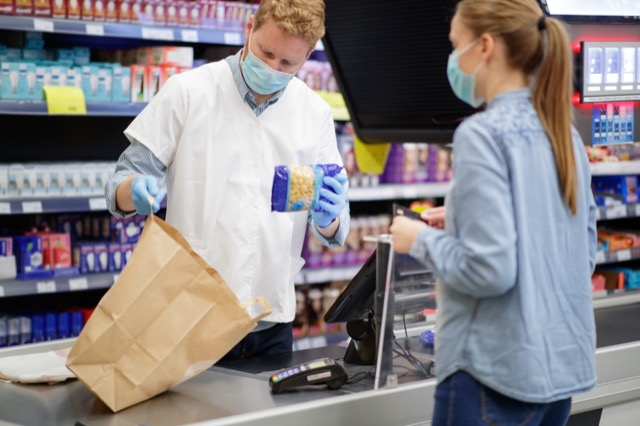
\includegraphics[height=3cm]{ex_27_img_1.png}
        \caption{the person with the ponytail [buys] stuff and other [packs] it}
        \end{subfigure}%    
        \caption*{\textit{Series}}
    \end{minipage}
    \hfill
    \begin{minipage}{.30\textwidth}
        \begin{subfigure}{\textwidth}
        \centering
        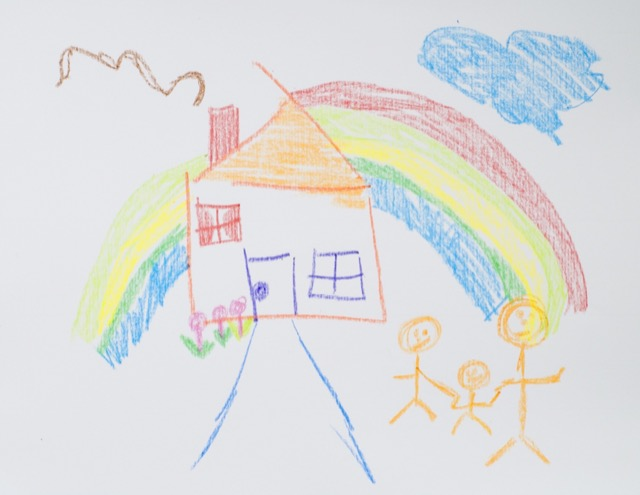
\includegraphics[height=3cm]{ex_61_img_0.png}
        \caption{there are [three] people and [two] windows}
        \end{subfigure}\\
        \begin{subfigure}{\textwidth}
        \centering
        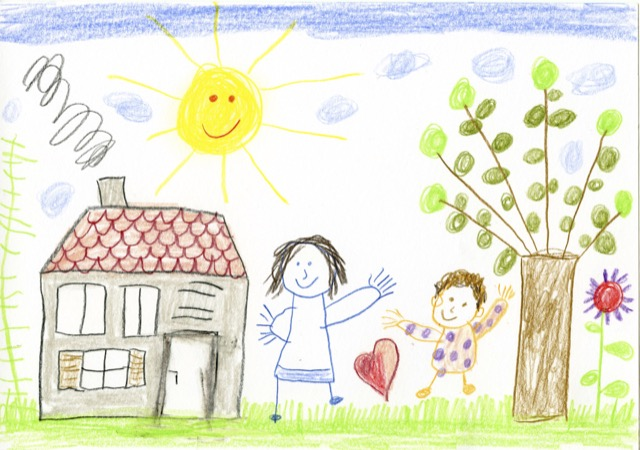
\includegraphics[height=3cm]{ex_61_img_1.png}
        \caption{there are [two] people and [three] windows}
        \end{subfigure}%    
        \caption*{\textit{Symbolic}}
    \end{minipage}
    \caption{Examples from the Winoground dataset for the visual tags \textit{Pragmatics}, \textit{Series} and \textit{Symbolic} from left to right. They are additionally tagged with the \textit{Relation} tag, and 1, 2, and 1 main predicate from left to right.}
    \label{fig:winoground-examples-visual}
\end{figure}

Winoground is a probing dataset so it prioritizes expert annotations over size. Therefore, there is no training split, all examples are used to evaluate models. The dataset has 400 examples, with 800 unique captions and images. These contain 1600 image-text pairs in total,
with 800 correct and 800 incorrect pairings.

\section{Metrics} \label{sec:winoground_metrics}

An example in Winoground is composed of two caption-image pairs: $(C_{0},I_{0})$ and $(C_{1},I_{1})$. Metrics must measure models' abilities to match pairs correctly. We compute two types of metrics, \textbf{score} and \textbf{accuracy}.

\paragraph{Score.}
Performance on Winoground \cite{thrush2022winoground} is computed according to three different score metrics that evaluate different aspects of the models' visio-linguistic reasoning abilities.

The first metric is the \textbf{text score}, which measures whether a model can select the correct caption, given an image:
\begin{equation}\label{eq:text-score}
        ts(C_{0},I_{0},C_{1},I_{1})= 
    \begin{cases}
        1 & \text{if}\  s(C_{0}, I_{0}) > s(C_{1}, I_{0}) \\
        & \ \ \text{and}\ s(C_{1}, I_{1}) > s(C_{0}, I_{1}) \\
        0              & \text{otherwise}
    \end{cases}
\end{equation}

The second metric is the \textbf{image score}, which measures whether a model can select the correct image, given a caption:
\begin{equation}\label{eq:image-score}
        is(C_{0},I_{0},C_{1},I_{1})= 
    \begin{cases}
        1 & \text{if}\  s(C_{0}, I_{0}) > s(C_{0}, I_{1})\\
        & \ \ \text{and}\ s(C_{1}, I_{1}) > s(C_{1}, I_{0}) \\
        0              & \text{otherwise}
    \end{cases}
\end{equation}

Our final metric \textbf{group score} combines the previous two, which measures if every combination for a given example is correct:
\begin{equation}\label{eq:group-score}
        gs(C_{0},I_{0},C_{1},I_{1})= 
    \begin{cases}
        1 & \text{if}\  ts(C_{0},I_{0},C_{1},I_{1})  \\
         & \ \ \text{and}\ is(C_{0},I_{0},C_{1},I_{1})\\
        0              & \text{otherwise}
    \end{cases}
\end{equation}

\paragraph{Accuracy.}
We also add three additional accuracy metrics for additional information. These are similar to the previous ones, but the accuracy is 0.5 when one of the pairs is correct.

The \textbf{text accuracy} for an example is computed according to:
\begin{equation}\label{eq:text-accuracy}
        ta(C_{0},I_{0},C_{1},I_{1})= 
    \begin{cases}
        1 & \text{if}\  s(C_{0}, I_{0}) > s(C_{1}, I_{0}) \\
        & \ \ \text{and}\ s(C_{1}, I_{1}) > s(C_{0}, I_{1}) \\
        0.5 & \text{if}\  s(C_{0}, I_{0}) > s(C_{1}, I_{0}) \\
        & \ \ \text{xor}\ s(C_{1}, I_{1}) > s(C_{0}, I_{1}) \\
        0              & \text{otherwise}
    \end{cases}
\end{equation}

The \textbf{image accuracy} for an example is calculated according to:
\begin{equation}\label{eq:image-accuracy}
        ia(C_{0},I_{0},C_{1},I_{1})= 
    \begin{cases}
        1 & \text{if}\  s(C_{0}, I_{0}) > s(C_{0}, I_{1})\\
        & \ \ \text{and}\ s(C_{1}, I_{1}) > s(C_{1}, I_{0}) \\
        0.5 & \text{if}\  s(C_{0}, I_{0}) > s(C_{0}, I_{1})\\
        & \ \ \text{xor}\ s(C_{1}, I_{1}) > s(C_{1}, I_{0}) \\
        0              & \text{otherwise}
    \end{cases}
\end{equation}

The \textbf{group accuracy} in our framework is the mean of both accuracies:
\begin{equation}\label{eq:group-accuracy}
        ga(C_{0},I_{0},C_{1},I_{1})= 
        (ta(C_{0},I_{0},C_{1},I_{1}) + ia(C_{0},I_{0},C_{1},I_{1})) / 2\\
\end{equation}

\section{Experiments and Results} \label{sec:winoground_experiments_results}

\subsection{Compared To Humans}

\paragraph{Previous}

We show baseline results from previous experiments \cite{thrush2022winoground} in \cref{tab:results_aggr_baseline}, which includes the following multimodal transformers: CLIP \cite{radford2021clip}, FLAVA \cite{singh2022flava}, LXMERT \cite{tan2020lxmert}, UniT \cite{hu2021unit}, UNITER \cite{chen2020uniter}, VILLA \cite{gan2020villa}, VinVL \cite{zhang2021vinvl}, ViLT \cite{kim2021vilt}, VisualBERT \cite{li2019visualbert} and ViLBERT \cite{lu2019vilbert}. Several configurations of two types of RNN-based models are also included: VSE++ \cite{faghri2018vse} and VSRN \cite{li2019vsrn}.

\begin{table}[ht]
\centering
\begin{tabular}{l|rrr|rrr}
\toprule
 &
  \multicolumn{3}{c|}{{Score}} &
  \multicolumn{3}{c}{{Accuracy}} \\
 Model                               & Text           & Image          & Group          & Text       & Image      & Group      \\
\midrule
 MTurk Human                         & \textbf{89.50} & \textbf{88.50} & \textbf{85.50} & \textbf{93.75} & \textbf{93.88} & \textbf{93.81} \\
 Random Chance                       & 25.00          & 25.00          & 16.67          & 50.00          & 50.00          & 50.00          \\
 \midrule
 VinVL                        & \textbf{37.75} & 17.75          & 14.50          & \textbf{62.75} & \textbf{57.75} & \textbf{60.25} \\
 UNITER$_{large}$             & \textbf{38.00} & 14.00          & 10.50          & \textbf{63.25} & \textbf{55.75} & \textbf{59.50} \\
 UNITER$_{base}$              & \textbf{32.25} & 13.25          & 10.00          & \textbf{60.62} & \textbf{55.50} & \textbf{58.06} \\
 ViLLA$_{large}$              & \textbf{37.00} & 13.25          & 11.00          & \textbf{62.62} & \textbf{55.25} & \textbf{58.94} \\
 ViLLA$_{base}$               & \textbf{30.00} & 12.00          & 8.00           & \textbf{59.62} & \textbf{55.00} & \textbf{57.31} \\
 VisualBERT$_{base}$          & 15.50          & 2.50           & 1.50           & \textbf{50.50} & 49.88          & \textbf{50.19} \\
 ViLT (ViT-B/32)              & \textbf{34.75} & 14.00          & 9.25           & \textbf{60.50} & \textbf{55.38} & \textbf{57.94} \\
 LXMERT                       & 19.25          & 7.00           & 4.00           & \textbf{52.12} & \textbf{51.88} & \textbf{52.00} \\
 ViLBERT$_{base}$             & 23.75          & 7.25           & 4.75           & \textbf{57.25} & \textbf{52.50} & \textbf{54.87} \\
 UniT$_{ITM Finetuned}$       & 19.50          & 6.25           & 4.00           & \textbf{50.25} & \textbf{50.75} & \textbf{50.50} \\
 FLAVA$_{ITM}$                & \textbf{32.25} & 20.50          & 14.25          & \textbf{62.75} & \textbf{59.13} & \textbf{60.94} \\
 FLAVA$_{ITC}$        & \textbf{25.25} & 13.50          & 9.00           & \textbf{59.25} & \textbf{55.12} & \textbf{57.19} \\
 CLIP (ViT-B/32)              & \textbf{30.75} & 10.50          & 8.00           & \textbf{60.38} & \textbf{53.25} & \textbf{56.81} \\
 VSE++$_{COCO}$ (ResNet)      & 22.75          & 8.00           & 4.00           & \textbf{51.38} & \textbf{50.88} & \textbf{51.12} \\
 VSE++$_{COCO}$ (VGG)         & 18.75          & 5.50           & 3.50           & \textbf{50.38} & 49.75          & \textbf{50.06} \\
 VSE++$_{Flickr30k}$ (ResNet) & 20.00          & 5.00           & 2.75           & \textbf{51.50} & \textbf{50.25} & \textbf{50.88} \\
 VSE++$_{Flickr30k}$ (VGG)    & 19.75          & 6.25           & 4.50           & \textbf{52.75} & \textbf{51.00} & \textbf{51.88} \\
 VSRN$_{COCO}$                & 17.50          & 7.00           & 3.75           & \textbf{50.38} & \textbf{51.12} & \textbf{50.75} \\
 VSRN$_{Flickr30k}$           & 20.00          & 5.00           & 3.50           & \textbf{53.25} & \textbf{51.75} & \textbf{52.50} \\
\bottomrule
\end{tabular}
\caption{Results on the Winoground dataset across the text, image and group score and accuracy metrics. Results above random chance in \textbf{bold}.}
\label{tab:results_aggr_baseline}
\end{table}

\textbf{Human performance} was computed using crowd workers on the Amazon Mechanical Turk platform. This establishes a more conservative human baseline than the expert annotator's perfect score \cite{thrush2022winoground}. Annotators are shown one image and one caption at a time and have to decide if they match. All 1600 combinations of images and captions are labelled by at least ten annotators. The image-caption score is computed as the ratio of annotators who say that they match.

\cref{tab:results_aggr_baseline} shows that there is a large \textbf{performance gap} between humans and models. On the one hand, \textbf{human performance} is high in all metrics, between 85\% and 90\% in \textbf{scores} and around 93\% in \textbf{accuracy}. On the other hand, most models perform below random chance in all scores and slightly above random chance in accuracy.

First, only some models are above random chance in \textbf{text score}: UNITER, VILLA, VinVL, ViLT, FLAVA, and CLIP. The larger versions of UNITER and VILLA, and VinVL are the models that perform best, and there is still more than 50\% difference with human performance.

Second, the performance on \textbf{image score} is even worse, where no model performs better than random chance. In contrast, text and image scores in humans are nearly the same. Even the best performing models (FLAVA$_{ITM}$ and VinVL) have nearly 70\% difference with the human score.

Last, \textbf{group score} is also below random chance for all models, while it is only a bit lower than other scores for humans. Similar to the image score, there is a 70\% difference between the human score and the best models, which are again FLAVA$_{ITM}$ and VinVL.

\paragraph{Ours}
We show our results in \cref{tab:results_aggr_ours}, which includes various configurations of the following multimodal transformers: OFA \cite{wang2022unifying}, BLIP \cite{li2022blip}, CLIP \cite{radford2021clip}, FLAVA \cite{singh2022flava} and ViLT \cite{kim2021vilt}. OFA and BLIP were not included in the previous experiments. The other models were already included but we test more configurations. For example, we test ViLT models that are finetuned on Flickr30k, COCO, NLVR2 and VSR. All the models except ViLT$_{VSR}$ are already fine-tuned and publicly available.

\begin{table}[ht]
\centering
\begin{tabular}{l|rrr|rrr}
\toprule
 &
  \multicolumn{3}{c|}{{Score}} &
  \multicolumn{3}{c}{{Accuracy}} \\
 Model                               & Text           & Image          & Group          & Text       & Image      & Group      \\
\midrule
 MTurk Human                         & \textbf{89.50} & \textbf{88.50} & \textbf{85.50} & \textbf{93.75} & \textbf{93.88} & \textbf{93.81} \\
 Random Chance                       & 25.00          & 25.00          & 16.67          & 50.00          & 50.00          & 50.00          \\
 \midrule
 ViLT (ViT-B/32)                     & \textbf{27.50} & 8.75           & 6.00           & \textbf{56.88} & \textbf{53.12} & \textbf{55.00} \\
 ViLT$_{COCO}$ (ViT-B/32)            & \textbf{32.75} & 13.50          & 11.25          & \textbf{61.88} & \textbf{56.00} & \textbf{58.94} \\
 ViLT$_{Flickr30k}$ (ViT-B/32)       & \textbf{35.00} & 11.50          & 9.75           & \textbf{61.62} & \textbf{54.50} & \textbf{58.06} \\
 ViLT$_{NLVR2}$ (ViT-B/32)           & \textbf{38.00} & 15.25          & 12.00          & \textbf{58.75} & \textbf{55.62} & \textbf{57.19} \\
 ViLT$_{VSR}$ Random (ViT-B/32)      & \textbf{30.50} & 14.50          & 8.00           & \textbf{59.00} & \textbf{55.75} & \textbf{57.38} \\
 ViLT$_{VSR}$ Zero-shot (ViT-B/32)   & \textbf{29.50} & 14.00          & 9.25           & \textbf{58.38} & \textbf{54.75} & \textbf{56.56} \\
 FLAVA$_{ITM}$                       & \textbf{32.25} & 20.50          & 14.25          & \textbf{62.75} & \textbf{59.13} & \textbf{60.94} \\
 FLAVA$_{ITC}$                       & \textbf{25.25} & 13.50          & 9.00           & \textbf{59.25} & \textbf{55.12} & \textbf{57.19} \\
 CLIP (ViT-B/32)                     & \textbf{30.75} & 10.25          & 8.25           & \textbf{60.38} & \textbf{53.12} & \textbf{56.75} \\
 CLIP (ViT-B/16)                     & 25.00          & 10.25          & 7.00           & \textbf{57.88} & \textbf{53.75} & \textbf{55.81} \\
 CLIP (ViT-L/14)                     & \textbf{28.50} & 11.00          & 8.00           & \textbf{60.38} & \textbf{54.62} & \textbf{57.50} \\
 CLIP (ViT-L/14-336)                 & \textbf{27.50} & 12.00          & 8.00           & \textbf{59.38} & \textbf{55.12} & \textbf{57.25} \\
 OFA$_{Tiny}$                        & 20.50          & 8.00           & 3.75           & \textbf{53.50} & \textbf{52.00} & \textbf{52.75} \\
 OFA$_{Base}$                        & \textbf{26.50} & 10.50          & 7.00           & \textbf{58.88} & \textbf{54.00} & \textbf{56.44} \\
 OFA$_{Medium}$                      & 22.75          & 9.00           & 5.50           & \textbf{54.25} & \textbf{52.75} & \textbf{53.50} \\
 OFA$_{Large}$                       & \textbf{26.00} & 8.75           & 5.75           & \textbf{58.38} & \textbf{52.88} & \textbf{55.62} \\
 OFA$_{Huge}$                        & \textbf{36.25} & 15.50          & 13.50          & \textbf{64.38} & \textbf{56.62} & \textbf{60.50} \\
 BLIP$_{ITM 14M}$ (ViT-B/16)         & \textbf{39.25} & 19.00          & 15.00          & \textbf{65.88} & \textbf{58.25} & \textbf{62.06} \\
 BLIP$_{ITC 14M}$ (ViT-B/16)         & \textbf{32.25} & 13.75          & 10.50          & \textbf{62.25} & \textbf{56.50} & \textbf{59.38} \\
 BLIP$_{ITM}$ (ViT-B/16)             & \textbf{40.50} & 20.50          & 16.50          & \textbf{66.25} & \textbf{59.00} & \textbf{62.62} \\
 BLIP$_{ITC}$ (ViT-B/16)             & \textbf{29.75} & 14.50          & 9.50           & \textbf{59.88} & \textbf{56.12} & \textbf{58.00} \\
 BLIP$_{ITM}$ (ViT-B/16) (CapFilt-L) & \textbf{37.50} & 18.50          & 14.00          & \textbf{65.00} & \textbf{59.13} & \textbf{62.06} \\
 BLIP$_{ITC}$ (ViT-B/16) (CapFilt-L) & \textbf{31.50} & 10.50          & 8.50           & \textbf{61.38} & \textbf{53.62} & \textbf{57.50} \\
 BLIP$_{ITM}$ (ViT-L/16)             & \textbf{42.50} & 18.25          & 15.50          & \textbf{66.88} & \textbf{57.25} & \textbf{62.06} \\
 BLIP$_{ITC}$ (ViT-L/16)             & \textbf{33.25} & 12.00          & 9.00           & \textbf{61.75} & \textbf{55.00} & \textbf{58.38} \\
 BLIP$_{ITM COCO}$ (ViT-B/16)        & \textbf{48.00} & 24.50          & \textbf{20.00} & \textbf{69.88} & \textbf{61.25} & \textbf{65.56} \\
 BLIP$_{ITC COCO}$ (ViT-B/16)        & \textbf{37.75} & 15.75          & 12.75          & \textbf{65.00} & \textbf{56.88} & \textbf{60.94} \\
 BLIP$_{ITM Flickr30k}$ (ViT-B/16)   & \textbf{46.25} & 24.25          & \textbf{21.25} & \textbf{69.25} & \textbf{60.62} & \textbf{64.94} \\
 BLIP$_{ITC Flickr30k}$ (ViT-B/16)   & \textbf{38.25} & 15.00          & 12.25          & \textbf{65.38} & \textbf{56.12} & \textbf{60.75} \\
 BLIP$_{ITM COCO}$ (ViT-L/16)        & \textbf{46.75} & 24.00          & \textbf{20.50} & \textbf{68.88} & \textbf{61.00} & \textbf{64.94} \\
 BLIP$_{ITC COCO}$ (ViT-L/16)        & \textbf{37.75} & 13.75          & 10.50          & \textbf{64.88} & \textbf{55.75} & \textbf{60.31} \\
 BLIP$_{ITM Flickr30k}$ (ViT-L/16)   & \textbf{45.00} & 24.75          & \textbf{20.50} & \textbf{68.62} & \textbf{60.50} & \textbf{64.56} \\
 BLIP$_{ITC Flickr30k}$ (ViT-L/16)   & \textbf{36.00} & 16.25          & 13.50          & \textbf{63.38} & \textbf{56.75} & \textbf{60.06} \\
 BLIP$_{NLVR2}$ (ViT-B/16)           & \textbf{40.25} & 25.00          & \textbf{18.50} & \textbf{64.62} & \textbf{61.62} & \textbf{63.12} \\
\bottomrule
\end{tabular}
\caption{Results on the Winoground dataset across the text, image and group score and accuracy metrics. Results above random chance in \textbf{bold}.}
\label{tab:results_aggr_ours}
\end{table}

In the baseline models, only pre-trained models are tested. We extend this by testing some models that are fine-tuned for specific tasks. Those tasks include image-text retrieval and visual reasoning. We compare pre-trained versions with fine-tuned versions of the same models. Our aim is to measure if scores improve by fine-tuning on related tasks.

Depending on the model and setting, the score for an image-text pair is calculated in a different way. For contrastive models, we use cosine similarity between image and text embeddings (CLIP). Other models use the softmaxed probability from the image-text-match classifier (ViLT). BLIP and FLAVA include both options, image-text contrastive (ITC) and image-text matching (ITM) scores. OFA is a generative model, so we have to use the probability of generating that the image and text match. For models fine-tuned on visual reasoning tasks, we take the probability of the True label as a score. Due to its generative nature, we decided to test OFA, hoping that it would have better spatial reasoning skills.

We test 6 different versions of \textbf{ViLT}. The first one is the pre-trained version, without finetuning. Two others are finetuned for retrieval on COCO and Flickr30k. The next one is finetuned for visual reasoning on NLVR2. The last two are finetuned on different splits of VSR. The best one is the one trained on NLVR2, which shows that finetuning on that task helps perform better on Winoground. VSR fine-tuning also increases scores, but not as much as NLVR2. Finetuning for retrieval is also helpful and improves the results of the pre-trained model. The score of the pre-trained model is lower than the baseline one.

For \textbf{FLAVA} and \textbf{CLIP} we manage to replicate baseline results. We also test 3 other OpenAI CLIP \cite{radford2021clip} models with different configurations and find that they all perform similar to the baseline configuration. Finally, we test some new \textbf{OpenCLIP} \cite{ilharco_gabriel_2021_5143773} models, that were trained on LAION-2B, a subset of LAION-5B \cite{schuhmann2022laionb} with English captions. These models perform slightly better than OpenAI CLIP models.

We test the 5 model sizes of \textbf{OFA}. Considering that this model gets state-of-the-art performance on many tasks, the performance is not very good. Even the biggest model is not better than the best baseline model. OFA is trained to generate "yes" or "no" when given an image and the text "Does the image describe <caption>?". This might explain why it does not perform that well on retrieval and Winoground.

We test many configurations of \textbf{BLIP}, which include different training sizes, scoring, vision transformer sizes and finetuning datasets. ITM score is better than ITC score in all the cases. Even the 14M pretrained-only model is better than all the previously tested models. Finetuning for retrieval on COCO and Flickr30k improves the results even more, reaching nearly above random performance in text, image and group scores. The best scores are much better than baseline models, ~10\% in text score, ~4\% in image score and ~7\% in group score.

However, even the best model is still far from human performance in text, image and group scores. There is still a ~40\% gap in text scores, and ~64\% in image and group scores. If we look at accuracy metrics, the gap is reduced, but the difference is still very big. Image score remains much lower than text score for all the models.

\subsection{Results By Linguistic Tag}

\paragraph{Previous}

\cref{tab:results-by-ling-tag-baseline} shows results from previous experiments \cite{thrush2022winoground} by linguistic tags. The highest \textbf{human performance} for \textbf{swap-dependent linguistic tags} is on \textbf{object}, followed by \textbf{relation} and then \textbf{both}. For the \textbf{swap-independent linguistic tags}, humans do better on examples with two main predicates, which tend to be longer and more complicated.

\textbf{Models} perform much worse in all tags, but they show the \textbf{opposite pattern}. They perform better on examples with simpler and shorter sentences which often have morpheme-level swaps. Examples with the \textbf{both} tag have some of the shortest and least compositional captions. Many models get better than random performance on this tag, and CLIP even reaches human performance on text score. Image score remains lower than text score for all tags and models.

\begin{table}[ht]
    \centering
    \begin{adjustbox}{max width=\textwidth}
  \begin{tabular}{l|rrr|rrr|rrr|rrr|rrr}
    \toprule
     &
      \multicolumn{3}{c|}{Object} &
      \multicolumn{3}{c|}{Relation} &
      \multicolumn{3}{c|}{Both} &
      \multicolumn{3}{c|}{1 Main Pred} &
      \multicolumn{3}{c}{2 Main Preds}\\
    Model & Text & Image & Group & Text & Image & Group & Text & Image & Group & Text & Image & Group & Text & Image & Group \\\midrule
 MTurk Human                  & \textbf{92.20} & \textbf{90.78} & \textbf{88.65} & \textbf{89.27} & \textbf{90.56} & \textbf{86.70} & \textbf{76.92} & \textbf{57.69} & \textbf{57.69} & \textbf{87.33} & \textbf{85.62} & \textbf{82.53} & \textbf{95.37} & \textbf{96.30} & \textbf{93.52} \\
 VinVL                        & \textbf{36.88} & 17.73          & 14.18          & \textbf{37.77} & 17.60          & 14.16          & \textbf{42.31} & 19.23          & \textbf{19.23} & \textbf{39.38} & 21.23          & \textbf{17.47} & \textbf{33.33} & 8.33           & 6.48           \\
 UNITER$_{large}$             & \textbf{39.01} & 12.77          & 9.93           & \textbf{36.05} & 14.16          & 9.87           & \textbf{50.00} & 19.23          & \textbf{19.23} & \textbf{40.07} & 16.44          & 13.36          & \textbf{32.41} & 7.41           & 2.78           \\
 UNITER$_{base}$              & \textbf{34.04} & 11.35          & 9.22           & \textbf{30.04} & 14.16          & 10.30          & \textbf{42.31} & 15.38          & 11.54          & \textbf{35.27} & 14.73          & 11.99          & 24.07          & 9.26           & 4.63           \\
 ViLLA$_{large}$              & \textbf{36.88} & 14.89          & 11.35          & \textbf{37.34} & 12.88          & 11.16          & \textbf{34.62} & 7.69           & 7.69           & \textbf{39.73} & 17.12          & 14.38          & \textbf{29.63} & 2.78           & 1.85           \\
 ViLLA$_{base}$               & \textbf{33.33} & 15.60          & 9.93           & \textbf{27.04} & 9.01           & 6.01           & \textbf{38.46} & 19.23          & 15.38          & \textbf{33.22} & 14.04          & 10.27          & 21.30          & 6.48           & 1.85           \\
 VisualBERT$_{base}$          & 19.15          & 2.13           & 0.71           & 12.88          & 2.15           & 1.72           & 19.23          & 7.69           & 3.85           & 16.44          & 2.74           & 1.71           & 12.96          & 1.85           & 0.93           \\
 ViLT (ViT-B/32)              & \textbf{31.91} & 15.60          & 9.22           & \textbf{36.91} & 11.59          & 8.15           & \textbf{30.77} & \textbf{26.92} & \textbf{19.23} & \textbf{35.27} & 17.12          & 11.64          & \textbf{33.33} & 5.56           & 2.78           \\
 LXMERT                       & 22.70          & 9.22           & 6.38           & 17.60          & 5.58           & 2.58           & 15.38          & 7.69           & 3.85           & 19.18          & 8.56           & 5.14           & 19.44          & 2.78           & 0.93           \\
 ViLBERT$_{base}$             & \textbf{29.08} & 10.64          & 7.09           & 19.31          & 3.00           & 1.72           & \textbf{34.62} & \textbf{26.92} & \textbf{19.23} & 23.97          & 8.90           & 5.82           & 23.15          & 2.78           & 1.85           \\
 UniT$_{ITM finetuned}$       & 17.73          & 5.67           & 2.13           & 18.03          & 4.72           & 3.43           & \textbf{42.31} & 23.08          & \textbf{19.23} & 21.58          & 6.85           & 4.11           & 13.89          & 4.63           & 3.70           \\
  FLAVA$_{ITM}$                & \textbf{31.91} & 23.40 & 14.89 & \textbf{30.04} & 16.31 & 12.02 & \textbf{53.85} & \textbf{42.31} & \textbf{30.77} & \textbf{36.30} & 24.66 & \textbf{17.81} & 21.30          & 9.26 & 4.63 \\
 FLAVA$_{ITC}$        & 23.40          & 19.15 & 11.35 & 23.61          &  8.58 &  5.58 & \textbf{50.00} & \textbf{26.92} & \textbf{26.92} & \textbf{26.37} & 16.44 & 10.62          & 22.22          &  5.56 & 4.63 \\
 CLIP (ViT-B/32)              & \textbf{34.75} & 7.80           & 6.38           & 22.75          & 8.58           & 5.58           & \textbf{80.77} & \textbf{42.31} & \textbf{38.46} & \textbf{35.27} & 13.01          & 10.27          & 18.52          & 3.70           & 1.85           \\
 VSE++$_{COCO}$ (ResNet)      & 21.99          & 6.38           & 1.42           & 23.61          & 9.01           & 5.58           & 19.23          & 7.69           & 3.85           & 25.00          & 9.59           & 4.79           & 16.67          & 3.70           & 1.85           \\
 VSE++$_{COCO}$ (VGG)         & 17.73          & 2.13           & 2.13           & 18.45          & 7.30           & 3.86           & \textbf{26.92} & 7.69           & 7.69           & 18.49          & 4.79           & 2.74           & 19.44          & 7.41           & 5.56           \\
 VSE++$_{Flickr30k}$ (ResNet) & 20.57          & 6.38           & 3.55           & 18.88          & 4.29           & 2.15           & \textbf{26.92} & 3.85           & 3.85           & 21.58          & 6.51           & 3.42           & 15.74          & 0.93           & 0.93           \\
 VSE++$_{Flickr30k}$ (VGG)    & 17.73          & 4.96           & 2.84           & 19.74          & 6.87           & 5.15           & \textbf{30.77} & 7.69           & 7.69           & 20.55          & 6.16           & 4.79           & 17.59          & 6.48           & 3.70           \\
 VSRN$_{COCO}$                & 15.60          & 4.96           & 2.13           & 18.88          & 7.73           & 4.72           & 15.38          & 11.54          & 3.85           & 17.12          & 7.19           & 3.77           & 18.52          & 6.48           & 3.70           \\
 VSRN$_{Flickr30k}$           & 16.31          & 4.96           & 2.13           & 21.03          & 4.29           & 3.86           & \textbf{30.77} & 11.54          & 7.69           & 20.89          & 5.82           & 3.77           & 17.59          & 2.78           & 2.78           \\
          \bottomrule
  \end{tabular}
  \end{adjustbox}
  \caption{The results by linguistic tag. Results above chance are in \textbf{bold}.}
    \label{tab:results-by-ling-tag-baseline}
\end{table}

\paragraph{Ours}

See \cref{tab:results-by-ling-tag-ours}

\begin{table}[ht]
    \centering
    \begin{adjustbox}{max width=\textwidth}
  \begin{tabular}{l|rrr|rrr|rrr|rrr|rrr}
    \toprule
     &
      \multicolumn{3}{c|}{Object} &
      \multicolumn{3}{c|}{Relation} &
      \multicolumn{3}{c|}{Both} &
      \multicolumn{3}{c|}{1 Main Pred} &
      \multicolumn{3}{c}{2 Main Preds}\\
    Model & Text & Image & Group & Text & Image & Group & Text & Image & Group & Text & Image & Group & Text & Image & Group \\\midrule
 MTurk Human                  & \textbf{92.20} & \textbf{90.78} & \textbf{88.65} & \textbf{89.27} & \textbf{90.56} & \textbf{86.70} & \textbf{76.92} & \textbf{57.69} & \textbf{57.69} & \textbf{87.33} & \textbf{85.62} & \textbf{82.53} & \textbf{95.37} & \textbf{96.30} & \textbf{93.52} \\
 ViLT (ViT-B/32)                     & \textbf{29.08} & 10.64          & 4.96           & \textbf{26.18} & 7.73           & 6.44           & \textbf{30.77} & 7.69           & 7.69           & \textbf{30.14} & 10.62          & 7.53           & 20.37          & 3.70           & 1.85           \\
 ViLT$_{COCO}$ (ViT-B/32)            & \textbf{33.33} & 15.60          & 12.77          & \textbf{30.90} & 10.73          & 9.01           & \textbf{46.15} & \textbf{26.92} & \textbf{23.08} & \textbf{36.64} & 15.75          & 14.04          & 22.22          & 7.41           & 3.70           \\
 ViLT$_{Flickr30k}$ (ViT-B/32)       & \textbf{32.62} & 14.89          & 11.35          & \textbf{35.62} & 8.15           & 7.73           & \textbf{42.31} & 23.08          & \textbf{19.23} & \textbf{36.99} & 14.38          & 11.99          & \textbf{29.63} & 3.70           & 3.70           \\
 ViLT$_{NLVR2}$ (ViT-B/32)           & \textbf{39.01} & 16.31          & 14.18          & \textbf{36.48} & 14.59          & 10.30          & \textbf{46.15} & 15.38          & 15.38          & \textbf{39.73} & 18.15          & 15.07          & \textbf{33.33} & 7.41           & 3.70           \\
 ViLT$_{VSR}$ Random (ViT-B/32)      & \textbf{34.75} & 17.73          & 9.93           & \textbf{27.47} & 11.16          & 6.01           & \textbf{34.62} & \textbf{26.92} & 15.38          & \textbf{32.53} & 16.44          & 9.59           & 25.00          & 9.26           & 3.70           \\
 ViLT$_{VSR}$ Zero-shot (ViT-B/32)   & \textbf{34.75} & 19.86          & 14.18          & \textbf{26.18} & 10.73          & 6.44           & \textbf{30.77} & 11.54          & 7.69           & \textbf{32.19} & 15.75          & 11.30          & 22.22          & 9.26           & 3.70           \\
 FLAVA$_{ITM}$                       & \textbf{31.91} & 23.40          & 14.89          & \textbf{30.04} & 16.31          & 12.02          & \textbf{53.85} & \textbf{42.31} & \textbf{30.77} & \textbf{36.30} & 24.66          & \textbf{17.81} & 21.30          & 9.26           & 4.63           \\
 FLAVA$_{ITC}$                       & 23.40          & 19.15          & 11.35          & 23.61          & 8.58           & 5.58           & \textbf{50.00} & \textbf{26.92} & \textbf{26.92} & \textbf{26.37} & 16.44          & 10.62          & 22.22          & 5.56           & 4.63           \\
 CLIP (ViT-B/32)                     & \textbf{35.46} & 7.80           & 6.38           & 22.32          & 7.73           & 5.58           & \textbf{80.77} & \textbf{46.15} & \textbf{42.31} & \textbf{35.62} & 13.01          & 10.62          & 17.59          & 2.78           & 1.85           \\
 CLIP (ViT-B/16)                     & \textbf{27.66} & 10.64          & 5.67           & 19.31          & 6.44           & 4.29           & \textbf{61.54} & \textbf{42.31} & \textbf{38.46} & \textbf{30.14} & 11.99          & 8.90           & 11.11          & 5.56           & 1.85           \\
 CLIP (ViT-L/14)                     & \textbf{27.66} & 8.51           & 5.67           & \textbf{25.75} & 9.87           & 6.44           & \textbf{57.69} & \textbf{34.62} & \textbf{34.62} & \textbf{30.14} & 13.01          & 9.93           & 24.07          & 5.56           & 2.78           \\
 CLIP (ViT-L/14-336)                 & \textbf{32.62} & 12.77          & 9.22           & 21.03          & 8.15           & 4.29           & \textbf{57.69} & \textbf{42.31} & \textbf{34.62} & \textbf{30.48} & 14.04          & 10.62          & 19.44          & 6.48           & 0.93           \\
 OFA$_{Tiny}$                        & 22.70          & 6.38           & 2.13           & 17.17          & 6.87           & 3.43           & \textbf{38.46} & \textbf{26.92} & 15.38          & 23.97          & 8.22           & 4.45           & 11.11          & 7.41           & 1.85           \\
 OFA$_{Base}$                        & \textbf{25.53} & 14.18          & 7.09           & 24.46          & 6.87           & 5.15           & \textbf{50.00} & 23.08          & \textbf{23.08} & \textbf{28.77} & 12.67          & 8.56           & 20.37          & 4.63           & 2.78           \\
 OFA$_{Medium}$                      & 19.86          & 7.80           & 4.26           & 22.32          & 7.73           & 4.72           & \textbf{42.31} & \textbf{26.92} & \textbf{19.23} & 24.32          & 10.96          & 6.85           & 18.52          & 3.70           & 1.85           \\
 OFA$_{Large}$                       & \textbf{26.24} & 10.64          & 5.67           & 24.03          & 5.15           & 3.86           & \textbf{42.31} & \textbf{30.77} & \textbf{23.08} & \textbf{29.45} & 10.96          & 7.53           & 16.67          & 2.78           & 0.93           \\
 OFA$_{Huge}$                        & \textbf{40.43} & 18.44          & 15.60          & \textbf{30.90} & 11.59          & 9.87           & \textbf{61.54} & \textbf{34.62} & \textbf{34.62} & \textbf{39.73} & 19.18          & \textbf{16.78} & \textbf{26.85} & 5.56           & 4.63           \\
 BLIP$_{ITM 14M}$ (ViT-B/16)         & \textbf{41.84} & 23.40          & \textbf{17.73} & \textbf{36.05} & 14.59          & 11.59          & \textbf{53.85} & \textbf{34.62} & \textbf{30.77} & \textbf{43.84} & 23.63          & \textbf{18.49} & \textbf{26.85} & 6.48           & 5.56           \\
 BLIP$_{ITC 14M}$ (ViT-B/16)         & \textbf{34.04} & 13.48          & 9.93           & \textbf{28.33} & 12.02          & 9.44           & \textbf{57.69} & \textbf{30.77} & \textbf{23.08} & \textbf{37.67} & 16.44          & 13.01          & 17.59          & 6.48           & 3.70           \\
 BLIP$_{ITM}$ (ViT-B/16)             & \textbf{46.10} & 22.70          & \textbf{17.73} & \textbf{35.62} & 17.60          & 14.16          & \textbf{53.85} & \textbf{34.62} & \textbf{30.77} & \textbf{45.89} & \textbf{25.34} & \textbf{20.55} & \textbf{25.93} & 7.41           & 5.56           \\
 BLIP$_{ITC}$ (ViT-B/16)             & \textbf{34.75} & 14.18          & 9.22           & \textbf{25.32} & 13.73          & 8.58           & \textbf{42.31} & 23.08          & \textbf{19.23} & \textbf{33.56} & 16.10          & 10.62          & 19.44          & 10.19          & 6.48           \\
 BLIP$_{ITM}$ (ViT-B/16) (CapFilt-L) & \textbf{39.01} & 19.86          & 12.77          & \textbf{34.76} & 15.88          & 12.45          & \textbf{53.85} & \textbf{34.62} & \textbf{34.62} & \textbf{41.10} & 22.60          & \textbf{17.12} & \textbf{27.78} & 7.41           & 5.56           \\
 BLIP$_{ITC}$ (ViT-B/16) (CapFilt-L) & \textbf{36.88} & 12.77          & 9.22           & \textbf{26.18} & 8.58           & 7.30           & \textbf{50.00} & 15.38          & 15.38          & \textbf{35.96} & 13.36          & 10.96          & 19.44          & 2.78           & 1.85           \\
 BLIP$_{ITM}$ (ViT-L/16)             & \textbf{41.84} & 19.86          & \textbf{17.02} & \textbf{40.77} & 16.31          & 13.73          & \textbf{61.54} & \textbf{26.92} & \textbf{23.08} & \textbf{45.55} & 23.29          & \textbf{20.21} & \textbf{34.26} & 4.63           & 2.78           \\
 BLIP$_{ITC}$ (ViT-L/16)             & \textbf{34.04} & 14.18          & 11.35          & \textbf{30.90} & 9.01           & 6.01           & \textbf{50.00} & \textbf{26.92} & \textbf{23.08} & \textbf{36.99} & 14.04          & 10.96          & 23.15          & 6.48           & 3.70           \\
 BLIP$_{ITM COCO}$ (ViT-B/16)        & \textbf{42.55} & \textbf{26.95} & \textbf{19.15} & \textbf{49.79} & 21.89          & \textbf{19.31} & \textbf{61.54} & \textbf{34.62} & \textbf{30.77} & \textbf{48.97} & \textbf{29.79} & \textbf{24.66} & \textbf{45.37} & 10.19          & 7.41           \\
 BLIP$_{ITC COCO}$ (ViT-B/16)        & \textbf{36.88} & 19.15          & 14.18          & \textbf{36.05} & 11.59          & 10.30          & \textbf{57.69} & \textbf{34.62} & \textbf{26.92} & \textbf{41.78} & 18.84          & 15.07          & \textbf{26.85} & 7.41           & 6.48           \\
 BLIP$_{ITM Flickr30k}$ (ViT-B/16)   & \textbf{49.65} & \textbf{28.37} & \textbf{22.70} & \textbf{42.49} & 19.74          & \textbf{18.45} & \textbf{61.54} & \textbf{42.31} & \textbf{38.46} & \textbf{51.03} & \textbf{28.42} & \textbf{26.03} & \textbf{33.33} & 12.96          & 8.33           \\
 BLIP$_{ITC Flickr30k}$ (ViT-B/16)   & \textbf{36.88} & 17.02          & 10.64          & \textbf{36.48} & 12.02          & 11.16          & \textbf{61.54} & \textbf{30.77} & \textbf{30.77} & \textbf{40.75} & 17.12          & 13.70          & \textbf{31.48} & 9.26           & 8.33           \\
 BLIP$_{ITM COCO}$ (ViT-L/16)        & \textbf{48.94} & \textbf{25.53} & \textbf{20.57} & \textbf{44.64} & 22.32          & \textbf{20.60} & \textbf{53.85} & \textbf{30.77} & \textbf{19.23} & \textbf{51.03} & \textbf{28.42} & \textbf{23.97} & \textbf{35.19} & 12.04          & 11.11          \\
 BLIP$_{ITC COCO}$ (ViT-L/16)        & \textbf{36.88} & 14.18          & 11.35          & \textbf{36.05} & 11.16          & 7.30           & \textbf{57.69} & \textbf{34.62} & \textbf{34.62} & \textbf{41.10} & 16.44          & 13.36          & \textbf{28.70} & 6.48           & 2.78           \\
 BLIP$_{ITM Flickr30k}$ (ViT-L/16)   & \textbf{46.10} & 22.70          & 16.31          & \textbf{42.06} & 24.89          & \textbf{21.46} & \textbf{65.38} & \textbf{34.62} & \textbf{34.62} & \textbf{50.34} & \textbf{29.11} & \textbf{24.66} & \textbf{30.56} & 12.96          & 9.26           \\
 BLIP$_{ITC Flickr30k}$ (ViT-L/16)   & \textbf{39.01} & 19.86          & 15.60          & \textbf{30.47} & 11.59          & 9.44           & \textbf{69.23} & \textbf{38.46} & \textbf{38.46} & \textbf{39.38} & 20.55          & \textbf{17.12} & \textbf{26.85} & 4.63           & 3.70           \\
 BLIP$_{NLVR2}$ (ViT-B/16)           & \textbf{42.55} & 23.40          & \textbf{19.86} & \textbf{36.48} & \textbf{25.32} & \textbf{16.74} & \textbf{61.54} & \textbf{30.77} & \textbf{26.92} & \textbf{42.47} & \textbf{27.74} & \textbf{21.23} & \textbf{34.26} & 17.59          & 11.11    \\
          \bottomrule
  \end{tabular}
  \end{adjustbox}
  \caption{The results by linguistic tag. Results above chance are in \textbf{bold}.}
    \label{tab:results-by-ling-tag-ours}
\end{table}

\subsection{Results By Visual Tag}

\paragraph{Previous}

See \cref{tab:results-by-visual-tag-baseline}

\begin{table}[ht]
    \centering
   \begin{adjustbox}{max width=\textwidth}
  \begin{tabular}{l|rrr|rrr|rrr}
    \toprule
     &
      \multicolumn{3}{c|}{Symbolic} &
      \multicolumn{3}{c|}{Pragmatics} &
      \multicolumn{3}{c}{Same Image Series} \\
    Model & Text & Image & Group & Text & Image & Group & Text & Image & Group \\\midrule
 MTurk Human                  & \textbf{96.43} & \textbf{92.86} & \textbf{92.86} & \textbf{58.82} & \textbf{41.18} & \textbf{41.18} & \textbf{95.65} & \textbf{91.30} & \textbf{91.30} \\
 VinVL                        & 25.00          & 17.86          & 14.29          & \textbf{29.41} & 5.88           & 5.88           & \textbf{34.78} & 17.39          & 13.04          \\
 UNITER$_{large}$             & \textbf{39.29} & \textbf{28.57} & \textbf{17.86} & \textbf{35.29} & 0.00           & 0.00           & 4.35           & 8.70           & 0.00           \\
 UNITER$_{base}$              & \textbf{46.43} & 14.29          & 14.29          & \textbf{29.41} & 17.65          & 11.76          & 8.70           & 8.70           & 0.00           \\
 ViLLA$_{large}$              & \textbf{39.29} & 14.29          & 10.71          & 17.65          & 0.00           & 0.00           & 17.39          & 4.35           & 0.00           \\
 ViLLA$_{base}$               & \textbf{42.86} & 17.86          & 14.29          & \textbf{29.41} & 5.88           & 5.88           & 13.04          & 8.70           & 4.35           \\
 VisualBERT$_{base}$          & \textbf{28.57} & 0.00           & 0.00           & 5.88           & 0.00           & 0.00           & 13.04          & 0.00           & 0.00           \\
 ViLT (ViT-B/32)              & \textbf{28.57} & 17.86          & 10.71          & \textbf{35.29} & 0.00           & 0.00           & \textbf{26.09} & 0.00           & 0.00           \\
 LXMERT                       & \textbf{28.57} & 3.57           & 3.57           & 17.65          & 5.88           & 0.00           & 8.70           & 4.35           & 0.00           \\
 ViLBERT$_{base}$             & \textbf{28.57} & 10.71          & 7.14           & \textbf{29.41} & 5.88           & 5.88           & 13.04          & 0.00           & 0.00           \\
 UniT$_{ITM finetuned}$       & 14.29          & 10.71          & 7.14           & 17.65          & 5.88           & 5.88           & 21.74          & 4.35           & 4.35           \\
 FLAVA$_{ITM}$                & 25.00          & \textbf{28.57} & \textbf{17.86} & 17.65          & \textbf{29.41} & 11.76 & 17.39          &  8.70 &  0.00 \\
 FLAVA$_{ITC}$        & 17.86          & 10.71          & 10.71          & 11.76          & 23.53          & 5.88           & 17.39          & 4.35           &  4.35 \\
 CLIP (ViT-B/32)              & \textbf{39.29} & 3.57           & 3.57           & \textbf{35.29} & 5.88           & 5.88           & 8.70           & 0.00           & 0.00           \\
 VSE++$_{COCO}$ (ResNet)      & \textbf{32.14} & 10.71          & 10.71          & 23.53          & 11.76          & 0.00           & 13.04          & 4.35           & 4.35           \\
 VSE++$_{COCO}$ (VGG)         & 17.86          & 14.29          & 7.14           & 17.65          & 0.00           & 0.00           & 13.04          & 4.35           & 4.35           \\
 VSE++$_{Flickr30k}$ (ResNet) & 21.43          & 3.57           & 0.00           & 23.53          & 0.00           & 0.00           & 17.39          & 4.35           & 0.00           \\
 VSE++$_{Flickr30k}$ (VGG)    & \textbf{28.57} & 10.71          & 10.71          & 11.76          & 0.00           & 0.00           & 13.04          & 4.35           & 0.00           \\
 VSRN$_{COCO}$                & 7.14           & 3.57           & 0.00           & 11.76          & 0.00           & 0.00           & 13.04          & 0.00           & 0.00           \\
 VSRN$_{Flickr30k}$           & 21.43          & 3.57           & 3.57           & \textbf{35.29} & 11.76          & 5.88           & 8.70           & 4.35           & 4.35           \\
    \bottomrule
  \end{tabular}
  \end{adjustbox}
  \caption{The results by visual tag. Results above chance are in \textbf{bold}.}
    \label{tab:results-by-visual-tag-baseline}
\end{table}

\paragraph{Ours}

See \cref{tab:results-by-visual-tag-ours}

\begin{table}[ht]
    \centering
   \begin{adjustbox}{max width=\textwidth}
  \begin{tabular}{l|rrr|rrr|rrr}
    \toprule
     &
      \multicolumn{3}{c|}{Symbolic} &
      \multicolumn{3}{c|}{Pragmatics} &
      \multicolumn{3}{c}{Same Image Series} \\
    Model & Text & Image & Group & Text & Image & Group & Text & Image & Group \\\midrule
 MTurk Human                  & \textbf{96.43} & \textbf{92.86} & \textbf{92.86} & \textbf{58.82} & \textbf{41.18} & \textbf{41.18} & \textbf{95.65} & \textbf{91.30} & \textbf{91.30} \\
 ViLT (ViT-B/32)                     & 21.43          & 7.14           & 3.57           & 17.65          & 5.88           & 5.88           & 17.39          & 8.70           & 4.35           \\
 ViLT$_{COCO}$ (ViT-B/32)            & 21.43          & 10.71          & 10.71          & \textbf{29.41} & 17.65          & 5.88           & 21.74          & 8.70           & 4.35           \\
 ViLT$_{Flickr30k}$ (ViT-B/32)       & \textbf{28.57} & 7.14           & 7.14           & 23.53          & 0.00           & 0.00           & \textbf{26.09} & 4.35           & 4.35           \\
 ViLT$_{NLVR2}$ (ViT-B/32)           & \textbf{42.86} & 10.71          & 10.71          & \textbf{41.18} & 0.00           & 0.00           & 17.39          & 13.04          & 4.35           \\
 ViLT$_{VSR}$ Random (ViT-B/32)      & \textbf{28.57} & 14.29          & 7.14           & \textbf{29.41} & 11.76          & 5.88           & \textbf{30.43} & 21.74          & 8.70           \\
 ViLT$_{VSR}$ Zero-shot (ViT-B/32)   & 25.00          & 10.71          & 7.14           & \textbf{35.29} & 23.53          & 11.76          & \textbf{30.43} & 8.70           & 0.00           \\
 FLAVA$_{ITM}$                       & 25.00          & \textbf{28.57} & \textbf{17.86} & 17.65          & \textbf{29.41} & 11.76          & 17.39          & 8.70           & 0.00           \\
 FLAVA$_{ITC}$                       & 17.86          & 10.71          & 10.71          & 11.76          & 23.53          & 5.88           & 17.39          & 4.35           & 4.35           \\
 CLIP (ViT-B/32)                     & \textbf{35.71} & 3.57           & 3.57           & \textbf{35.29} & 5.88           & 5.88           & 13.04          & 0.00           & 0.00           \\
 CLIP (ViT-B/16)                     & 21.43          & 3.57           & 3.57           & \textbf{29.41} & 11.76          & 11.76          & 4.35           & 4.35           & 0.00           \\
 CLIP (ViT-L/14)                     & \textbf{28.57} & 10.71          & 3.57           & 23.53          & 17.65          & 11.76          & 13.04          & 8.70           & 4.35           \\
 CLIP (ViT-L/14-336)                 & \textbf{28.57} & 14.29          & 7.14           & 17.65          & 17.65          & 5.88           & 13.04          & 4.35           & 0.00           \\
 OFA$_{Tiny}$                        & 21.43          & 7.14           & 7.14           & 11.76          & 17.65          & 0.00           & 21.74          & 8.70           & 0.00           \\
 OFA$_{Base}$                        & \textbf{28.57} & 10.71          & 10.71          & 23.53          & 5.88           & 5.88           & 21.74          & 13.04          & 4.35           \\
 OFA$_{Medium}$                      & \textbf{28.57} & 10.71          & 7.14           & 17.65          & 5.88           & 5.88           & 13.04          & 8.70           & 4.35           \\
 OFA$_{Large}$                       & \textbf{28.57} & 14.29          & 10.71          & \textbf{29.41} & 0.00           & 0.00           & 13.04          & 0.00           & 0.00           \\
 OFA$_{Huge}$                        & \textbf{39.29} & 14.29          & 14.29          & 11.76          & 11.76          & 5.88           & 17.39          & 4.35           & 4.35           \\
 BLIP$_{ITM 14M}$ (ViT-B/16)         & \textbf{46.43} & 17.86          & \textbf{17.86} & \textbf{35.29} & 11.76          & 11.76          & 17.39          & 4.35           & 0.00           \\
 BLIP$_{ITC 14M}$ (ViT-B/16)         & \textbf{32.14} & 14.29          & 10.71          & \textbf{29.41} & 0.00           & 0.00           & 13.04          & 0.00           & 0.00           \\
 BLIP$_{ITM}$ (ViT-B/16)             & \textbf{50.00} & 17.86          & \textbf{17.86} & \textbf{29.41} & 5.88           & 5.88           & 13.04          & 4.35           & 0.00           \\
 BLIP$_{ITC}$ (ViT-B/16)             & \textbf{39.29} & 10.71          & 7.14           & 5.88           & 11.76          & 0.00           & 4.35           & 8.70           & 0.00           \\
 BLIP$_{ITM}$ (ViT-B/16) (CapFilt-L) & \textbf{42.86} & 17.86          & 14.29          & 23.53          & 17.65          & \textbf{17.65} & 17.39          & 4.35           & 0.00           \\
 BLIP$_{ITC}$ (ViT-B/16) (CapFilt-L) & \textbf{42.86} & 0.00           & 0.00           & 17.65          & 0.00           & 0.00           & 4.35           & 0.00           & 0.00           \\
 BLIP$_{ITM}$ (ViT-L/16)             & \textbf{53.57} & 25.00          & \textbf{25.00} & \textbf{29.41} & 5.88           & 0.00           & \textbf{26.09} & 4.35           & 0.00           \\
 BLIP$_{ITC}$ (ViT-L/16)             & \textbf{39.29} & 17.86          & 14.29          & \textbf{41.18} & 11.76          & 11.76          & 8.70           & 4.35           & 4.35           \\
 BLIP$_{ITM COCO}$ (ViT-B/16)        & \textbf{53.57} & 17.86          & \textbf{17.86} & \textbf{58.82} & 17.65          & \textbf{17.65} & \textbf{39.13} & 8.70           & 0.00           \\
 BLIP$_{ITC COCO}$ (ViT-B/16)        & 25.00          & 10.71          & 7.14           & \textbf{35.29} & 5.88           & 5.88           & 17.39          & 8.70           & 4.35           \\
 BLIP$_{ITM Flickr30k}$ (ViT-B/16)   & \textbf{53.57} & 21.43          & \textbf{21.43} & \textbf{35.29} & 11.76          & 11.76          & \textbf{26.09} & 4.35           & 4.35           \\
 BLIP$_{ITC Flickr30k}$ (ViT-B/16)   & \textbf{35.71} & 10.71          & 10.71          & 23.53          & 17.65          & 11.76          & 17.39          & 4.35           & 0.00           \\
 BLIP$_{ITM COCO}$ (ViT-L/16)        & \textbf{39.29} & \textbf{35.71} & \textbf{25.00} & \textbf{58.82} & 23.53          & \textbf{17.65} & \textbf{26.09} & 4.35           & 0.00           \\
 BLIP$_{ITC COCO}$ (ViT-L/16)        & \textbf{46.43} & 14.29          & 14.29          & 17.65          & 5.88           & 5.88           & 13.04          & 0.00           & 0.00           \\
 BLIP$_{ITM Flickr30k}$ (ViT-L/16)   & \textbf{39.29} & \textbf{28.57} & \textbf{25.00} & \textbf{47.06} & 11.76          & 5.88           & \textbf{30.43} & 8.70           & 4.35           \\
 BLIP$_{ITC Flickr30k}$ (ViT-L/16)   & \textbf{39.29} & 14.29          & 14.29          & \textbf{47.06} & 5.88           & 5.88           & 21.74          & 13.04          & 13.04          \\
 BLIP$_{NLVR2}$ (ViT-B/16)           & \textbf{57.14} & 21.43          & 10.71          & \textbf{41.18} & 5.88           & 5.88           & 21.74          & 17.39          & 4.35           \\
\bottomrule
\end{tabular}
  \end{adjustbox}
  \caption{The results by visual tag. Results above chance are in \textbf{bold}.}
    \label{tab:results-by-visual-tag-ours}
\end{table}

\if0
\section{Discussion} \label{sec:winoground_disussion}

\subsection{Capabilities of Encoders}

\paragraph{Previous}

See \cref{tab:perplexity-and-length-correlations-baseline}

\begin{table}[ht]
\centering
\begin{adjustbox}{max width=\textwidth}
\begin{tabular}{l|rr|rrrrrr}
\toprule
 & \multicolumn{2}{c|}{Perplexity} &  \multicolumn{6}{c}{Caption Length}\\
 & \multicolumn{2}{c|}{Text-Image} &  \multicolumn{2}{c}{Text} &  \multicolumn{2}{c}{Image} &  \multicolumn{2}{c}{Group}\\
 Model      &   Corr. &   p-value & Corr. &   p-value & Corr. &   p-value & Corr. &   p-value\\\midrule 
  MTurk Human                  & 0.05           & 0.07          & \textbf{0.11}  & \textbf{0.03} & \textbf{0.20}  & \textbf{0.00} & \textbf{0.20}  & \textbf{0.00} \\
 VinVL                        & \textbf{-0.05} & \textbf{0.04} & \textbf{-0.11} & \textbf{0.03} & \textbf{-0.18} & \textbf{0.00} & \textbf{-0.20} & \textbf{0.00} \\
 UNITER$_{large}$             & -0.01          & 0.57          & -0.08          & 0.13          & -0.06          & 0.20          & \textbf{-0.16} & \textbf{0.00} \\
 UNITER$_{base}$              & -0.03          & 0.22          & \textbf{-0.15} & \textbf{0.00} & \textbf{-0.11} & \textbf{0.03} & \textbf{-0.14} & \textbf{0.00} \\
 ViLLA$_{large}$              & -0.02          & 0.39          & -0.05          & 0.32          & \textbf{-0.13} & \textbf{0.01} & \textbf{-0.12} & \textbf{0.01} \\
 ViLLA$_{base}$               & -0.04          & 0.13          & \textbf{-0.14} & \textbf{0.01} & \textbf{-0.12} & \textbf{0.01} & \textbf{-0.11} & \textbf{0.03} \\
 VisualBERT$_{base}$          & -0.04          & 0.15          & -0.09          & 0.07          & -0.07          & 0.14          & -0.06          & 0.22          \\
 ViLT (ViT-B/32)              & -0.04          & 0.16          & -0.09          & 0.06          & \textbf{-0.20} & \textbf{0.00} & \textbf{-0.16} & \textbf{0.00} \\
 LXMERT                       & -0.04          & 0.12          & -0.00          & 0.97          & -0.05          & 0.32          & \textbf{-0.11} & \textbf{0.02} \\
 ViLBERT$_{base}$             & -0.04          & 0.11          & -0.09          & 0.09          & \textbf{-0.15} & \textbf{0.00} & \textbf{-0.14} & \textbf{0.00} \\
 UniT$_{ITM Finetuned}$       & -0.01          & 0.73          & -0.03          & 0.53          & -0.05          & 0.32          & -0.02          & 0.73          \\
 FLAVA$_{ITM}$                & -0.03          & 0.22          & \textbf{-0.21} & \textbf{0.00} & \textbf{-0.22} & \textbf{0.00} & \textbf{-0.23} & \textbf{0.00} \\
 FLAVA$_{ITC}$        & \textbf{-0.06} & \textbf{0.01} & \textbf{-0.15} & \textbf{0.00} & \textbf{-0.25} & \textbf{0.00} & \textbf{-0.19} & \textbf{0.00} \\
 CLIP (ViT-B/32)              & -0.04          & 0.09          & \textbf{-0.27} & \textbf{0.00} & \textbf{-0.19} & \textbf{0.00} & \textbf{-0.22} & \textbf{0.00} \\
 VSE++$_{COCO}$ (ResNet)      & \textbf{-0.05} & \textbf{0.04} & -0.03          & 0.60          & -0.02          & 0.74          & 0.01           & 0.90          \\
 VSE++$_{COCO}$ (VGG)         & -0.04          & 0.08          & -0.02          & 0.65          & 0.03           & 0.50          & 0.03           & 0.56          \\
 VSE++$_{Flickr30k}$ (ResNet) & -0.02          & 0.43          & -0.01          & 0.80          & 0.01           & 0.91          & 0.02           & 0.67          \\
 VSE++$_{Flickr30k}$ (VGG)    & 0.01           & 0.74          & -0.09          & 0.07          & -0.07          & 0.18          & \textbf{-0.10} & \textbf{0.04} \\
 VSRN$_{COCO}$                & \textbf{-0.07} & \textbf{0.01} & -0.03          & 0.60          & -0.05          & 0.30          & -0.05          & 0.36          \\
 VSRN$_{Flickr30k}$           & -0.02          & 0.32          & -0.03          & 0.60          & -0.10          & 0.06          & -0.05          & 0.29          \\
\bottomrule
\end{tabular}
\end{adjustbox}
\caption{(left) The correlation between model image-caption scores and the caption perplexity from GPT2. (right) The correlation between the model text, image and group scores and the caption length.}
\label{tab:perplexity-and-length-correlations-baseline}
\end{table}

\paragraph{Ours}

See \cref{tab:perplexity-and-length-correlations-ours}

\begin{table}[ht]
\centering
\begin{adjustbox}{max width=\textwidth}
\begin{tabular}{l|rr|rrrrrr}
\toprule
 & \multicolumn{2}{c|}{Perplexity} &  \multicolumn{6}{c}{Caption Length}\\
 & \multicolumn{2}{c|}{Image-Caption} &  \multicolumn{2}{c}{Text} &  \multicolumn{2}{c}{Image} &  \multicolumn{2}{c}{Group}\\
 Model      &   Corr. &   p-value & Corr. &   p-value & Corr. &   p-value & Corr. &   p-value\\\midrule 
MTurk Human                         & 0.05           & 0.07          & \textbf{0.11}  & \textbf{0.03} & \textbf{0.20}  & \textbf{0.00} & \textbf{0.20}  & \textbf{0.00} \\
 ViLT (ViT-B/32)                     & -0.04          & 0.08          & \textbf{-0.12} & \textbf{0.02} & -0.07          & 0.17          & -0.05          & 0.35          \\
 ViLT$_{COCO}$ (ViT-B/32)            & -0.05          & 0.06          & \textbf{-0.21} & \textbf{0.00} & \textbf{-0.16} & \textbf{0.00} & \textbf{-0.17} & \textbf{0.00} \\
 ViLT$_{Flickr30k}$ (ViT-B/32)       & \textbf{-0.05} & \textbf{0.03} & \textbf{-0.11} & \textbf{0.03} & \textbf{-0.17} & \textbf{0.00} & \textbf{-0.14} & \textbf{0.01} \\
 ViLT$_{NLVR2}$ (ViT-B/32)           & 0.00           & 0.95          & \textbf{-0.13} & \textbf{0.01} & \textbf{-0.11} & \textbf{0.03} & \textbf{-0.12} & \textbf{0.02} \\
 FLAVA$_{ITM}$                       & -0.03          & 0.22          & \textbf{-0.21} & \textbf{0.00} & \textbf{-0.22} & \textbf{0.00} & \textbf{-0.23} & \textbf{0.00} \\
 FLAVA$_{ITC}$                       & \textbf{-0.06} & \textbf{0.01} & \textbf{-0.15} & \textbf{0.00} & \textbf{-0.25} & \textbf{0.00} & \textbf{-0.19} & \textbf{0.00} \\
 CLIP (ViT-B/32)                     & -0.04          & 0.10          & \textbf{-0.28} & \textbf{0.00} & \textbf{-0.21} & \textbf{0.00} & \textbf{-0.23} & \textbf{0.00} \\
 CLIP (ViT-B/16)                     & -0.04          & 0.11          & \textbf{-0.26} & \textbf{0.00} & \textbf{-0.22} & \textbf{0.00} & \textbf{-0.23} & \textbf{0.00} \\
 CLIP (ViT-L/14)                     & -0.03          & 0.22          & \textbf{-0.22} & \textbf{0.00} & \textbf{-0.17} & \textbf{0.00} & \textbf{-0.18} & \textbf{0.00} \\
 CLIP (ViT-L/14-336)                 & -0.04          & 0.11          & \textbf{-0.23} & \textbf{0.00} & \textbf{-0.22} & \textbf{0.00} & \textbf{-0.23} & \textbf{0.00} \\
 OFA$_{Tiny}$                        & -0.01          & 0.66          & \textbf{-0.17} & \textbf{0.00} & -0.06          & 0.24          & \textbf{-0.12} & \textbf{0.02} \\
 OFA$_{Base}$                        & -0.02          & 0.43          & \textbf{-0.15} & \textbf{0.00} & \textbf{-0.12} & \textbf{0.02} & \textbf{-0.10} & \textbf{0.05} \\
 OFA$_{Medium}$                      & -0.01          & 0.77          & \textbf{-0.11} & \textbf{0.03} & \textbf{-0.14} & \textbf{0.00} & \textbf{-0.12} & \textbf{0.01} \\
 OFA$_{Large}$                       & \textbf{-0.16} & \textbf{0.00} & \textbf{-0.18} & \textbf{0.00} & \textbf{-0.20} & \textbf{0.00} & \textbf{-0.17} & \textbf{0.00} \\
 OFA$_{Huge}$                        & 0.01           & 0.75          & \textbf{-0.15} & \textbf{0.00} & \textbf{-0.17} & \textbf{0.00} & \textbf{-0.16} & \textbf{0.00} \\
 BLIP$_{ITM 14M}$ (ViT-B/16)         & -0.00          & 0.85          & \textbf{-0.22} & \textbf{0.00} & \textbf{-0.23} & \textbf{0.00} & \textbf{-0.21} & \textbf{0.00} \\
 BLIP$_{ITC 14M}$ (ViT-B/16)         & -0.00          & 0.97          & \textbf{-0.24} & \textbf{0.00} & \textbf{-0.17} & \textbf{0.00} & \textbf{-0.17} & \textbf{0.00} \\
 BLIP$_{ITM}$ (ViT-B/16)             & \textbf{-0.05} & \textbf{0.04} & \textbf{-0.24} & \textbf{0.00} & \textbf{-0.23} & \textbf{0.00} & \textbf{-0.22} & \textbf{0.00} \\
 BLIP$_{ITC}$ (ViT-B/16)             & \textbf{-0.06} & \textbf{0.02} & \textbf{-0.19} & \textbf{0.00} & \textbf{-0.17} & \textbf{0.00} & \textbf{-0.13} & \textbf{0.01} \\
 BLIP$_{ITM}$ (ViT-B/16) (CapFilt-L) & \textbf{-0.10} & \textbf{0.00} & \textbf{-0.20} & \textbf{0.00} & \textbf{-0.28} & \textbf{0.00} & \textbf{-0.23} & \textbf{0.00} \\
 BLIP$_{ITC}$ (ViT-B/16) (CapFilt-L) & \textbf{-0.10} & \textbf{0.00} & \textbf{-0.25} & \textbf{0.00} & \textbf{-0.17} & \textbf{0.00} & \textbf{-0.15} & \textbf{0.00} \\
 BLIP$_{ITM}$ (ViT-L/16)             & \textbf{-0.07} & \textbf{0.01} & \textbf{-0.17} & \textbf{0.00} & \textbf{-0.21} & \textbf{0.00} & \textbf{-0.19} & \textbf{0.00} \\
 BLIP$_{ITC}$ (ViT-L/16)             & \textbf{-0.08} & \textbf{0.00} & \textbf{-0.22} & \textbf{0.00} & \textbf{-0.17} & \textbf{0.00} & \textbf{-0.17} & \textbf{0.00} \\
 BLIP$_{ITM COCO}$ (ViT-B/16)        & -0.04          & 0.11          & \textbf{-0.17} & \textbf{0.00} & \textbf{-0.26} & \textbf{0.00} & \textbf{-0.22} & \textbf{0.00} \\
 BLIP$_{ITC COCO}$ (ViT-B/16)        & \textbf{-0.06} & \textbf{0.02} & \textbf{-0.18} & \textbf{0.00} & \textbf{-0.26} & \textbf{0.00} & \textbf{-0.22} & \textbf{0.00} \\
 BLIP$_{ITM Flickr30k}$ (ViT-B/16)   & -0.04          & 0.11          & \textbf{-0.25} & \textbf{0.00} & \textbf{-0.28} & \textbf{0.00} & \textbf{-0.28} & \textbf{0.00} \\
 BLIP$_{ITC Flickr30k}$ (ViT-B/16)   & \textbf{-0.07} & \textbf{0.00} & \textbf{-0.20} & \textbf{0.00} & \textbf{-0.19} & \textbf{0.00} & \textbf{-0.18} & \textbf{0.00} \\
 BLIP$_{ITM COCO}$ (ViT-L/16)        & \textbf{-0.06} & \textbf{0.02} & \textbf{-0.24} & \textbf{0.00} & \textbf{-0.23} & \textbf{0.00} & \textbf{-0.23} & \textbf{0.00} \\
 BLIP$_{ITC COCO}$ (ViT-L/16)        & \textbf{-0.10} & \textbf{0.00} & \textbf{-0.21} & \textbf{0.00} & \textbf{-0.21} & \textbf{0.00} & \textbf{-0.21} & \textbf{0.00} \\
 BLIP$_{ITM Flickr30k}$ (ViT-L/16)   & \textbf{-0.05} & \textbf{0.04} & \textbf{-0.27} & \textbf{0.00} & \textbf{-0.25} & \textbf{0.00} & \textbf{-0.23} & \textbf{0.00} \\
 BLIP$_{ITC Flickr30k}$ (ViT-L/16)   & \textbf{-0.09} & \textbf{0.00} & \textbf{-0.24} & \textbf{0.00} & \textbf{-0.19} & \textbf{0.00} & \textbf{-0.16} & \textbf{0.00} \\
\bottomrule
\end{tabular}
\end{adjustbox}
\caption{(left) The correlation between model image-caption scores and the caption perplexity from GPT2. (right) The correlation between the model text, image and group scores and the caption length.}
\label{tab:perplexity-and-length-correlations-ours}
\end{table}

\subsection{By Multimodal Pretraining Dataset Size}

\paragraph{Previous}

See \cref{tab:data-size-correlations-baseline} and \cref{fig:pretraining_images_baseline}

\begin{table}[ht]
\centering
\begin{tabular}{llrr}
\toprule
Pretraining & Score & Corr. & p-value\\\midrule
 & Text & \textbf{0.84} & \textbf{0.00} \\
 Image & Image & \textbf{0.76} & \textbf{0.00} \\
 & Group & \textbf{0.75} & \textbf{0.00} \\\midrule
 & Text  & \textbf{0.77} & \textbf{0.00} \\
 Caption & Image & \textbf{0.75} & \textbf{0.00} \\
 & Group & \textbf{0.71} & \textbf{0.00} \\
\bottomrule
\end{tabular}
\caption{Correlations between the number of pretraining images and captions and the model text, image, and group scores. CLIP and FLAVA are excluded as outliers.}
\label{tab:data-size-correlations-baseline}
\end{table}

\begin{figure}[ht]
    \centering
    \subfloat{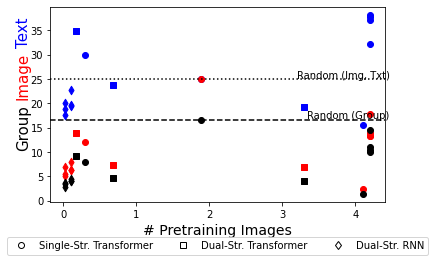
\includegraphics[width=0.49\linewidth]{images/winoground/pretraining_images_baseline.png}}
    \subfloat{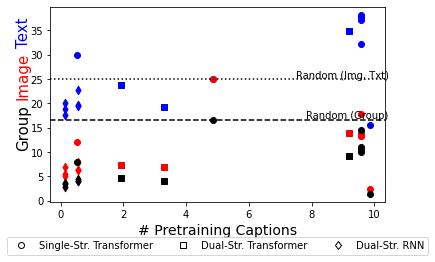
\includegraphics[width=0.49\linewidth]{images/winoground/pretraining_captions_baseline.png}}
    \caption{Graphs of the model performance on Winoground for each model by the number of pretraining images (left) and pretraining captions (right).}
    \label{fig:pretraining_images_baseline}
\end{figure}

\paragraph{Ours}

See \cref{tab:data-size-correlations-ours}  and \cref{fig:pretraining_images_ours}

\begin{table}[ht]
\centering
\begin{tabular}{llrr}
\toprule
Pretraining & Score & Corr. & p-value\\\midrule
               & Text    &  -0.09 &      0.65 \\
 Image              & Image   &  -0.16 &      0.44 \\
               & Group   &  -0.13 &      0.53 \\
             & Text    &  -0.09 &      0.66 \\
 Caption            & Image   &  -0.15 &      0.44 \\
             & Group   &  -0.12 &      0.54 \\
\bottomrule
\end{tabular}
\caption{Correlations between the number of pretraining images and captions and the model text, image, and group scores. Only BLIP, CLIP and FLAVA are included.}
\label{tab:data-size-correlations-ours}
\end{table}

\begin{figure}[ht]
    \centering
    \subfloat{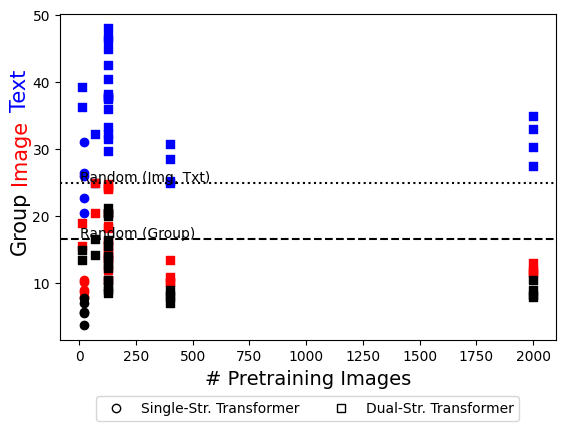
\includegraphics[width=0.49\linewidth]{images/winoground/pretraining_images_ours.png}}
    \subfloat{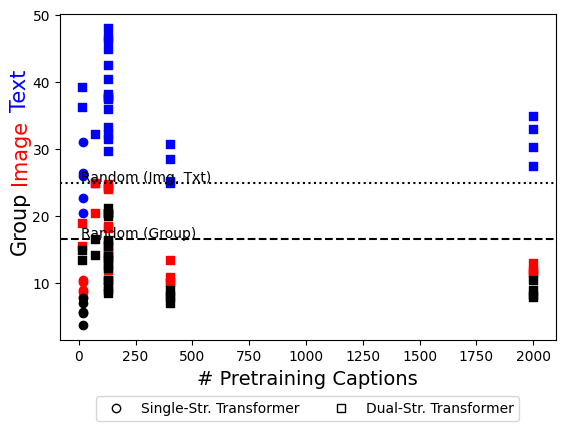
\includegraphics[width=0.49\linewidth]{images/winoground/pretraining_captions_ours.png}}
    \caption{Graphs of the model performance on Winoground for each model by the number of pretraining images (left) and pretraining captions (right).}
    \label{fig:pretraining_images_ours}
\end{figure}

\fi